%Talk given at Los Alamos National Labs 2019 July
\documentclass[10pt,compress,xcolor={usenames,dvipsnames},aspectratio=169]{beamer}
%\documentclass[xcolor={usenames,dvipsnames},aspectratio=169]{beamer} %slides and 
%notes
\usepackage{amsmath,datetime,
	mathtools,
	bbm,
	%mathabx,
	array,
	booktabs,
	xspace,
	calc,
	colortbl,
	scrextend,
 	graphicx}
\addtokomafont{labelinglabel}{\itshape\textcolor{IITred!80!IITgray}}
\usepackage[usenames]{xcolor}
\usepackage[giveninits=false,backend=biber,style=nature, maxcitenames =10, mincitenames=9]{biblatex}
\addbibresource{FJHown23.bib}
\addbibresource{FJH23.bib}
\usepackage{newpxtext}
\usepackage[euler-digits,euler-hat-accent]{eulervm}
\usepackage{media9}
\usepackage[autolinebreaks]{mcode}

\usetheme{FJHSlimNoFoot169}
\setlength{\parskip}{2ex}
\setlength{\arraycolsep}{0.5ex}

\newcommand{\contradiction}{%
  \ensuremath{{\Longrightarrow\mspace{-2mu}\Longleftarrow}}%
}

\DeclareMathOperator{\sol}{SOL}
\DeclareMathOperator{\app}{APP}
\DeclareMathOperator{\alg}{ALG}
\DeclareMathOperator{\ERR}{ERR}
\DeclareMathOperator{\COST}{COST}
\newcommand{\dataN}{\bigl(\hf(\vk_i)\bigr)_{i=1}^n}
\newcommand{\dataNj}{\bigl(\hf(\vk_i)\bigr)_{i=1}^{n_j}}
\newcommand{\dataNjd}{\bigl(\hf(\vk_i)\bigr)_{i=1}^{n_{j^\dagger}}}
\newcommand{\ERRN}{\ERR\bigl(\dataN,n\bigr)}

\newcommand{\Sapp}{S_{\textup{app}}}
\newcommand{\LambdaStd}{\Lambda^{\textup{std}}}
\newcommand{\LambdaSer}{\Lambda^{\textup{ser}}}
\newcommand{\LambdaAll}{\Lambda^{\textup{all}}}
%\DeclareMathOperator{\spann}{span}
%\DeclareMathOperator{\app}{app}

\providecommand{\HickernellFJ}{H.}


\iffalse
The Challenges of Approximating Functions of Many Variables
Fred J. Hickernell, Department of Applied Mathematics, Illinois Institute of Technology, Chicago, IL

Function approximation is relatively simple compared to many other continuous numerical problems, such as solving (stochastic and/or partial) differential equations. Interpolation is often used in the case of noiseless data, and regression can handle the case of noisy data.  For functions of one variable, collecting sufficient data is often straightforward, but for functions of many variables the function must satisfy some simplifying structure for approximation to be successful.  The problem is even more difficult when functions values are costly, such as when they are generated by some complex computer simulation.  This talk highlights some of the challenges of approximating functions of many variables and the strategies for overcoming these challenges.

\fi

\renewcommand{\OffTitleLength}{-10ex}
\setlength{\FJHThankYouMessageOffset}{-8ex}
\title{The Challenges of Approximating Functions of Many Variables}
\author[]{Fred J. Hickernell}
\institute{Department of Applied Mathematics \\
	Center for Interdisciplinary Scientific Computation \\  Illinois Institute of Technology \\
	\href{mailto:hickernell@iit.edu}{\url{hickernell@iit.edu}} \quad
	\href{http://mypages.iit.edu/~hickernell}{\url{mypages.iit.edu/~hickernell}}}

\thanksnote{Joint work with Yuhan Ding, Peter Kritzer, and Simon Mak \\
	This work partially supported by  NSF-DMS-1522687 and NSF-DMS-1638521 (SAMSI)
}
\event{Los Alamos National Laboratory}
\date[]{July 31, 2019}

\input FJHDef.tex


%Abstract:  When

\newlength{\figwidth}
\setlength{\figwidth}{0.25\textwidth}

\newlength{\figwidthSmall}
\setlength{\figwidthSmall}{0.2\textwidth}

\newcommand{\financePict}{\href{http://i2.cdn.turner.com/money/dam/assets/130611131918-chicago-board-options-exchange-1024x576.jpg}{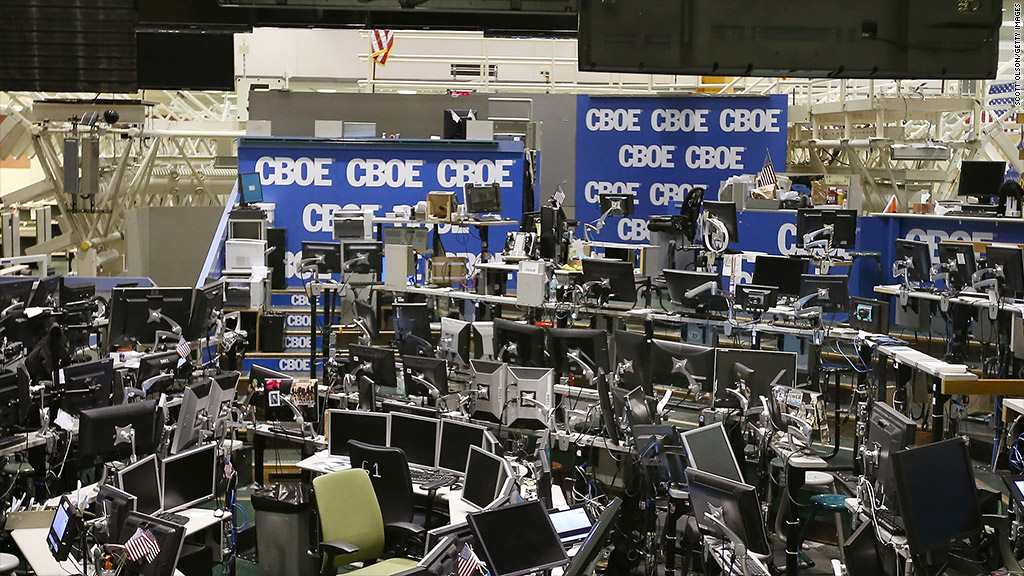
\includegraphics[width
		= 3cm]{ProgramsImages/130611131918-chicago-board-options-exchange-1024x576.jpg}}}
	
	\newcommand{\scoop}[1]{\parbox{#1}{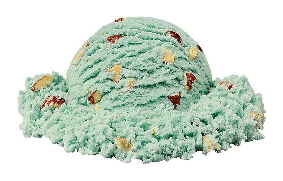
\includegraphics[width=#1]{IceCreamScoop.eps}}\xspace}
	\newcommand{\smallscoop}{\scoop{1cm}}
	\newcommand{\medscoop}{\scoop{1.8cm}}
	\newcommand{\largescoop}{\scoop{3cm}}
	\newcommand{\ICcone}[1]{\parbox{#1}{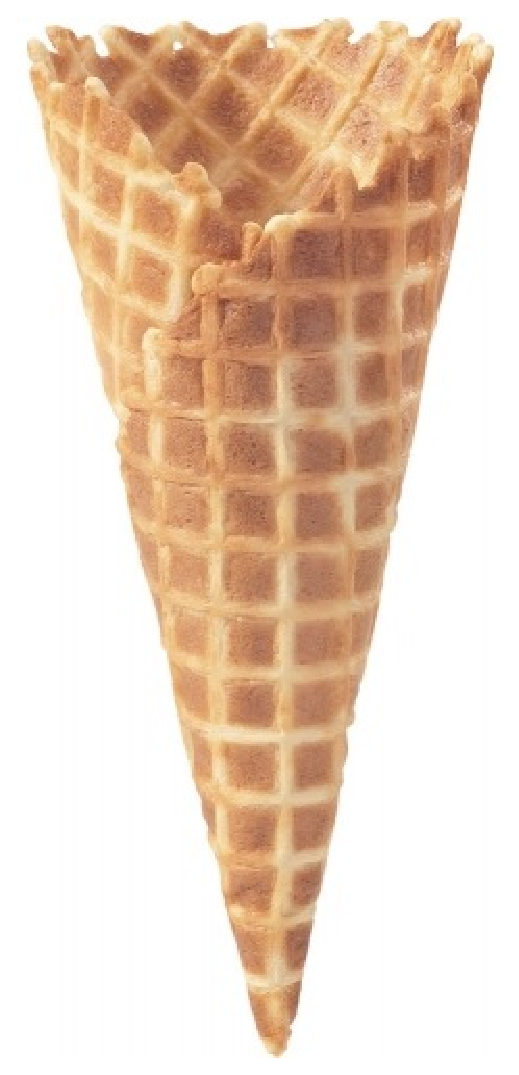
\includegraphics[width=#1,angle=270]{MediumWaffleCone.eps}}\xspace}
	\newcommand{\medcone}{\ICcone{1.2cm}}
	\newcommand{\largercone}{\parbox{2.2cm}{\vspace*{-0.2cm}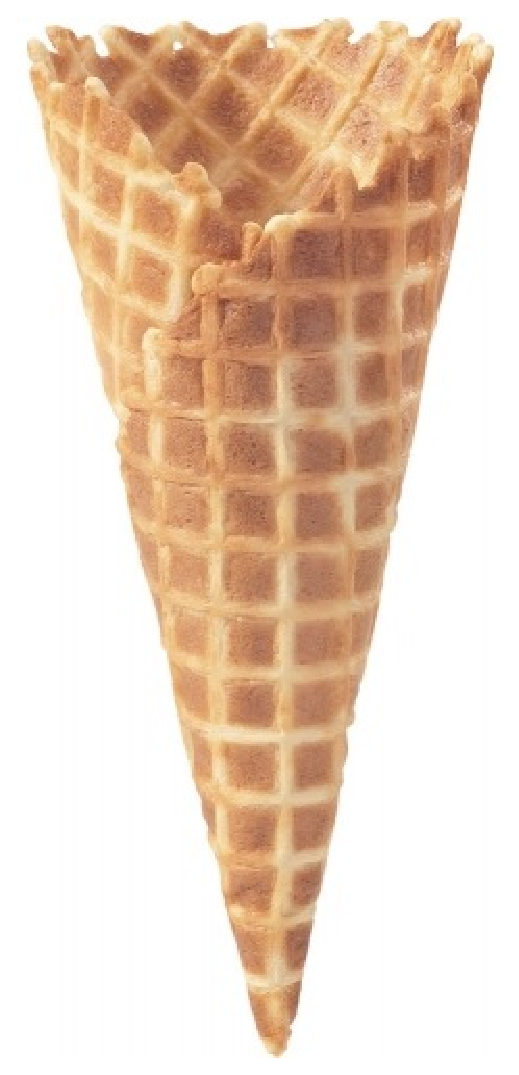
\includegraphics[width=1cm,angle=270]{MediumWaffleCone.eps}}\xspace}
	\newcommand{\largecone}{\ICcone{1.8cm}}
	\newcommand{\smallcone}{\parbox{1.1cm}{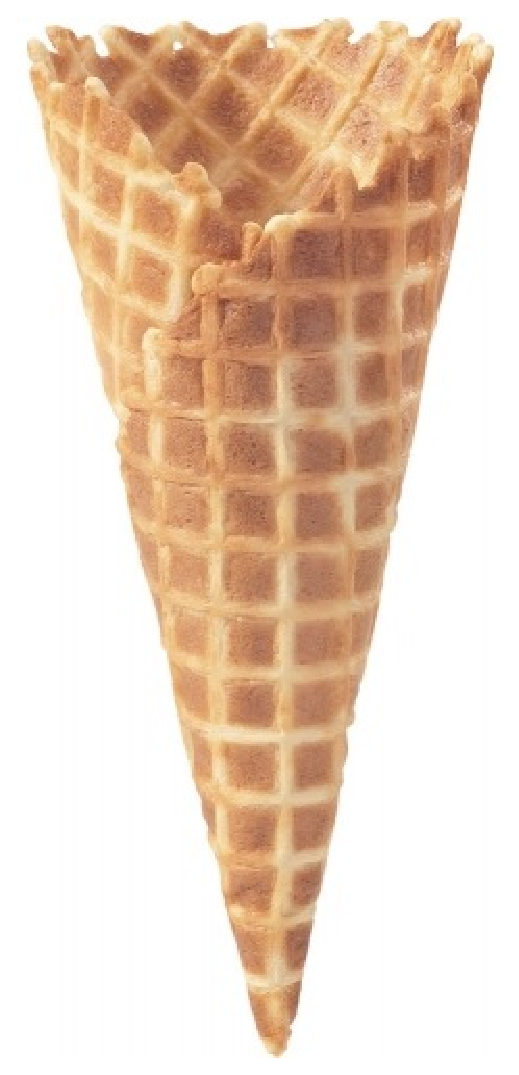
\includegraphics[width=0.5cm,angle=270]{MediumWaffleCone.eps}}\xspace}

	


\begin{document}
\everymath{\displaystyle}
\frame{\titlepage}

\section{Problem}

\begin{frame}{Problem}

\vspace{-5ex}

\begin{itemize}[]
    \item  Input
    \begin{addmargin}{3ex}
    \begin{labeling}{Error Tolerance}
       \item[\alert<1>{Black box}] providing \only<1>{\alert{noisy} or }\alert{noiseless} information about $f:\Omega \subseteq \reals^d \to \reals$
    \only<1-2>{ \\ e.g., function values or series coefficients,} \alert{costing} $\$(f)$ each
       \only<3->{\\ \alert<3>{$f \in \cf$, definition of $\norm[\cf]{\cdot}$ enshrines smoothness assumptions}}
        
        \item[\alert<1>{Error tolerance}] $\varepsilon$
     
    \end{labeling}
    \end{addmargin}
    \vspace{1ex}
    
    \item Output $\alg(f,\varepsilon)$ \only<1>{(as a surrogate, for solving PDEs, for uncertainty quantification) }that is
    \begin{addmargin}{3ex}
    \begin{labeling}{Accurate}
        \item[\alert<1>{Cheap}] to evaluate
        
        \item[\alert<1>{Accurate}] $\norm[\cg]{f - \alg(f,\varepsilon)} \le \varepsilon$ \uncover<4->{\quad \alert<4>{$\forall f \in \ch \subset \cf$}}
        
        \item[\alert<1>{Efficient}] to construct\uncover<5->{, \alert{$\COST(f,\varepsilon) = \Order( \varepsilon^{-p} R^p d^q)$ for $\norm[\cf]{f} \le R$ and optimal $p$ and $q$}}

    \end{labeling}
    \end{addmargin}
    \vspace{1ex}

	\item<2-> Approximation  with fixed computation budget: $\app(f,n) = \sum_{i=1}^n L_i(f) g_{i,n}$
	\setbeamertemplate{itemize items}[triangle]
	\begin{itemize}
	    \item $L_1(f), L_2(f), \ldots$ is input function information% 
	    \only<2>{, e.g., function values or series coefficients}
	    \item $\vg_n = (g_{1,n}, \ldots, g_{n,n}) \in \cg^n$
	    \item $ \alert{\COST(f,n)} = \Order(n \$(f) + \COST( \vg_n))$
	\end{itemize}
    \vspace{1ex}
	
	\item<2-> Algorithm $\alg(f,\varepsilon) = \app(f,n^*(f,\varepsilon))$ satisfying  
	$\norm[\cg]{f -  \app(f,n^*(f,\varepsilon))} \le \varepsilon$ \uncover<4->{\quad \alert<4>{$\forall f \in \ch \subset \cf$}}
	\setbeamertemplate{itemize items}[triangle]
		\begin{itemize}
	    \item $ \alert{\COST(f,\varepsilon)} = \COST(f,n^*(f,\varepsilon)) + \text{ cost to determine } n^*(f,\varepsilon)$
	\end{itemize}


\end{itemize}

\end{frame}

%%%%%%%%%%%%%%%%%%%%%%%%%%%%%%%%%%%%%%%%%%%%%%%%%%%%%%%%%%%%%%%%%%%%
\section{Solvability}
%%%%%%%%%%%%%%%%%%%%%%%%%%%%%%%%%%%%%%%%%%%%%%%%%%%%%%%%%%%%%%%%%%%%

\begin{frame}{Impossible for All $f$ in Infinite Dimensional $\cf$}
\vspace{-5ex}
\[
\norm[\cg]{f - \alg(f,\varepsilon)} \le \varepsilon \quad \forall f \in \ch \alert{\subset} \cf
\]
\alert{Proof by contradiction}

\vspace{-3ex}
\begin{itemize}
    \item Suppose $\ch = \cf$
    
    \item Fix $\varepsilon > 0$
    
    \item Let $L_1, \ldots, L_n$ be the information used to construct $\alg(0,\varepsilon)$
    
    \item Choose \alert{nonzero fooling function} $f \in \cf$, such that $L_1(f) = \cdots = L_n(f) = 0$
    
    \item $\alg(\pm cf,\varepsilon) = 0$ for all $c > 0$
    
    \item For all $c > 0$
    \begin{align*}
        \varepsilon & \ge \max\bigl(\norm[\cg]{cf - \alg(cf,\varepsilon)}, \norm[\cg]{-cf - \alg(cf,\varepsilon)} \bigr) \\
        & \ge \frac 12 \bigl(\norm[\cg]{cf - \alg(cf,\varepsilon)} + \norm[\cg]{cf + \alg(cf,\varepsilon)} \bigr) \\
        & \ge  c \norm[\cg]{f} \qquad \contradiction
    \end{align*}
    
\end{itemize}

\end{frame}

%%%%%%%%%%%%%%%%%%%%%%%%%%%%%%%%%%%%%%%%%%%%%%%%%%%%%%%%%%%%%%%%%%%%
\section{Smoothness}
%%%%%%%%%%%%%%%%%%%%%%%%%%%%%%%%%%%%%%%%%%%%%%%%%%%%%%%%%%%%%%%%%%%%

\begin{frame}<1>[label = smoothness]{Smoothness Makes Algorithm Less Expensive}
\vspace{-3ex}
For \alert{$d = 1$}, let $\{u_1, u_2, \ldots\}$ be an orthogonal (polynomial) basis for $\cf$ and $\cg$

\vspace{-6ex}
\begin{gather*}
    \cf := \left \{ f = \sum_{k=0}^\infty \hf(k) u_k  : \norm[\cf]{f} : = \norm[2]{\left(\frac{\hf(k)}{\lambda_k} \right)_{k=0}^\infty } < \infty \right \}, \qquad \lambda_1 \ge  \lambda_2 \ge \cdots > 0 \\
   \cg := \left \{ g = \sum_{k=0}^\infty \hg(k) u_k  : \norm[\cg]{g} : = \norm[2]{\bigl(\hg(k) \bigr)_{k=0}^\infty } < \infty \right \}, \qquad \app(f,n) = \sum_{k=0}^{n-1} \hf(k) u_{k} 
   \uncover<2->{\\
   \norm[\cg]{f - \app(f,n)} 
   = \norm[2]{\bigl(\hf(k) \bigr)_{k=n}^\infty } 
   = \norm[2]{\left(\frac{\lambda_k \, \hf(k)}{\lambda_k} \right)_{k=n}^\infty} \underbrace{\le}_{\text{tight}} \norm[\cf]{f} \lambda_{n} \alert{\overset{?}{\le}} \varepsilon, \quad \alert{\text{require } \lambda_n \downarrow 0}}
\end{gather*}

\uncover<3->{
\vspace{-3ex}
By choosing $\ch = \cb_R := \{ f \in \cf : \norm[\cf]{f} \le R\}$, we can define our \alert{algorithm}
\begin{gather*}
    \alg(f,\varepsilon) 
    = \app(f,n^*), \quad n^* = \min\{n : \lambda_{n} \le R/\varepsilon\}, \qquad
    \norm[\cg]{f - \alg(f,\varepsilon)} \le \varepsilon \quad \forall f \in \cb_R\\ 
    \lambda_n = \Order(n^{-1/p}) \implies \COST(\cb_R,\varepsilon) = \Order(R^p\varepsilon^{-p})
\end{gather*}
\vspace{-7ex}
\begin{itemize}
    \item<4-> $\alg$ has \alert{optimal} cost among all successful algorithms using Fourier coefficients \\
    (look at the cost of approximating the zero function)
    \item<5-> Similar results for algorithms based on \alert{function values}, but need to choose the \alert{design} carefully
\end{itemize}
}
    
\end{frame}

\begin{frame}{Bases for Function Approximation}
\vspace{-3ex}
	\begin{tabular}{>{\centering}m{0.18\textwidth}>{\centering}m{0.18\textwidth}>{\centering}m{0.18\textwidth}>{\centering}m{0.18\textwidth}>{\centering}m{0.18\textwidth}}
		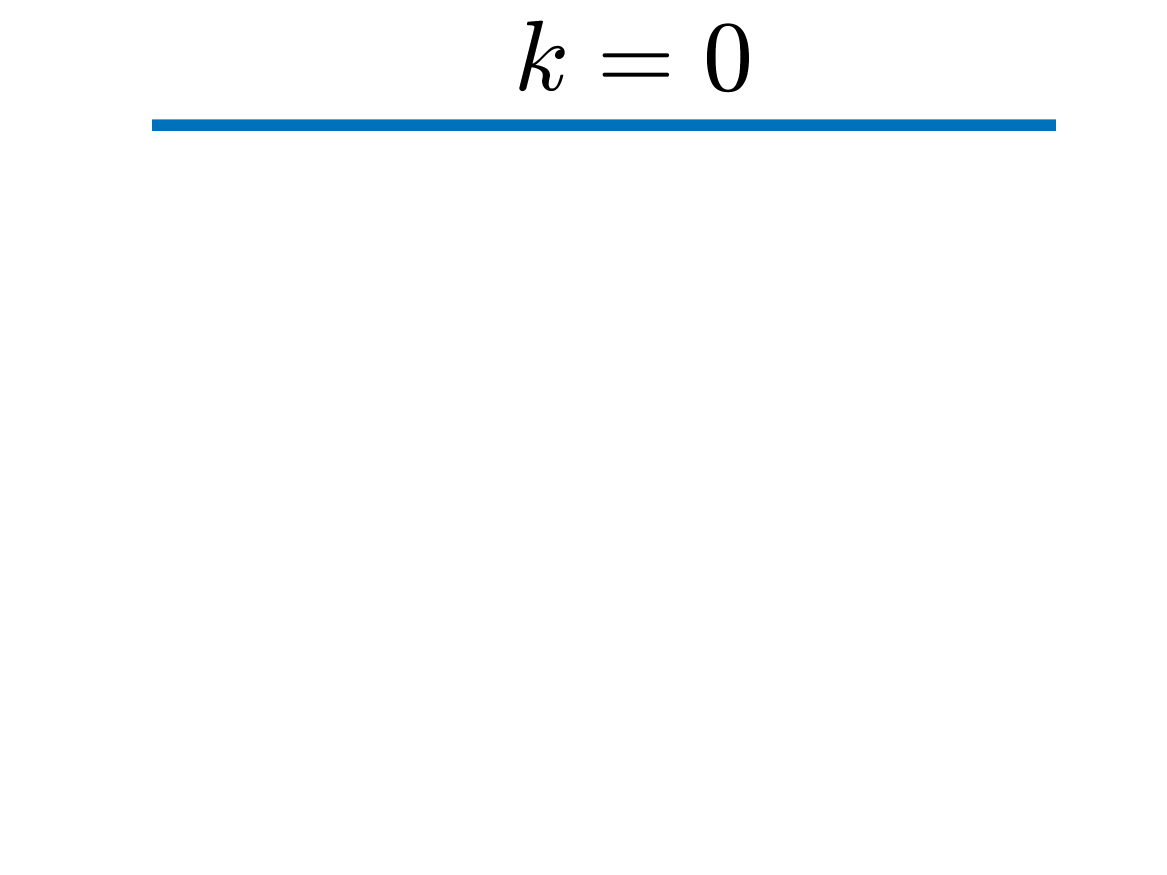
\includegraphics[width =0.18\textwidth]{ProgramsImages/Legendre_Degree_0_1D_k.png}  &
		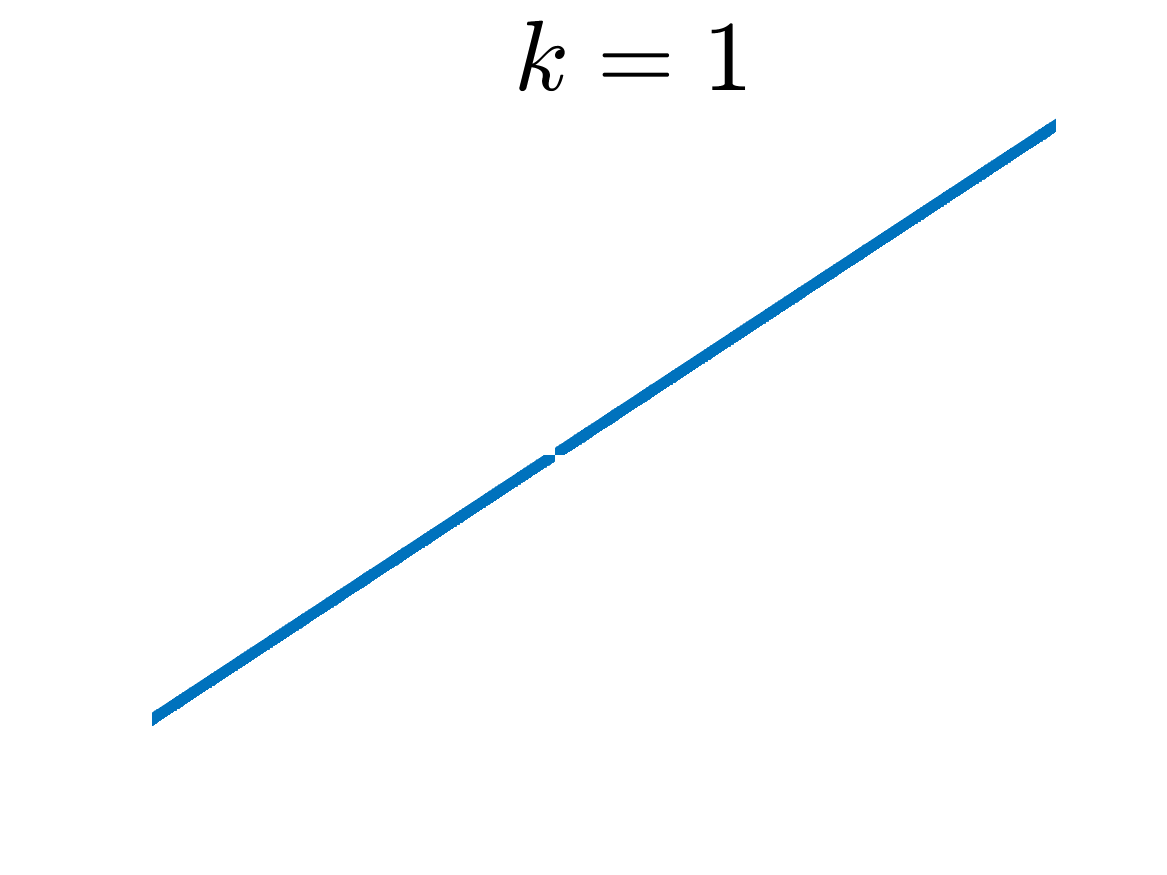
\includegraphics[width =0.18\textwidth]{ProgramsImages/Legendre_Degree_1_1D_k.png}  &
		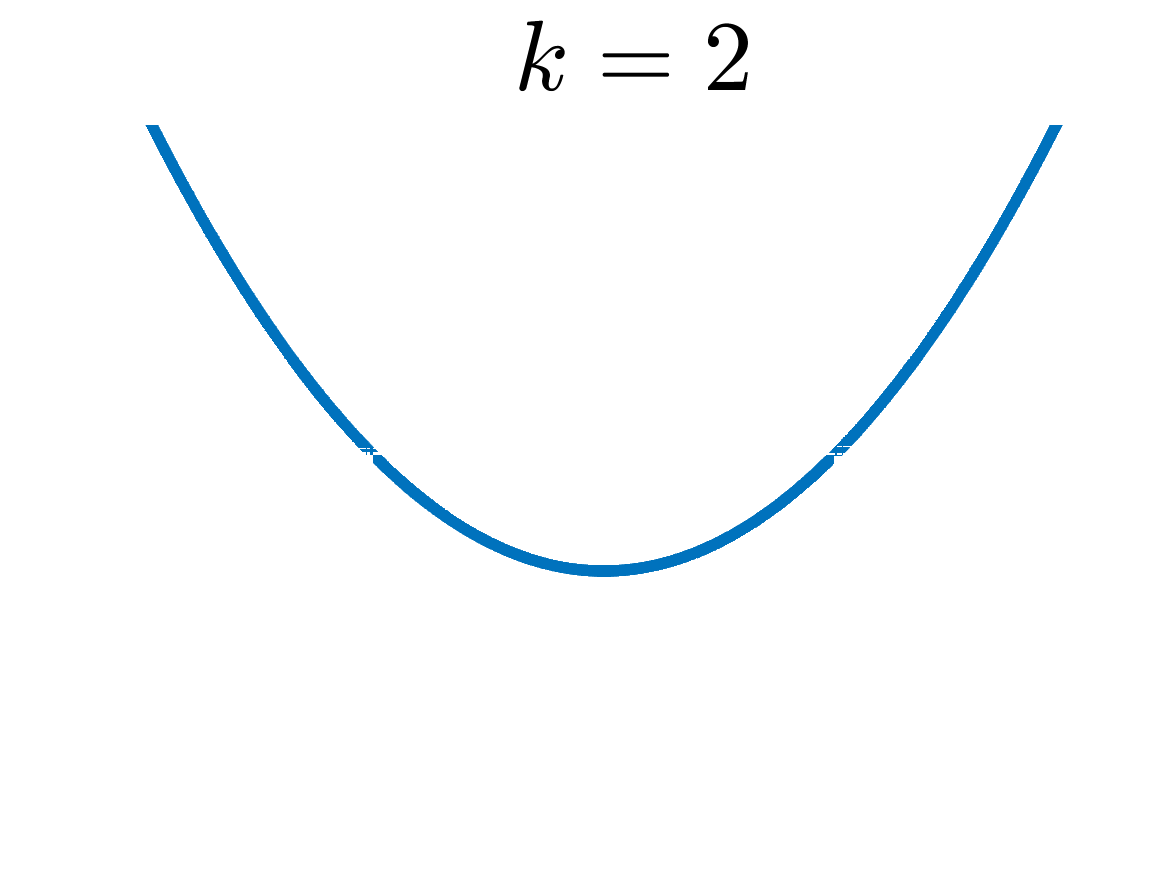
\includegraphics[width =0.18\textwidth]{ProgramsImages/Legendre_Degree_2_1D_k.png}  &
		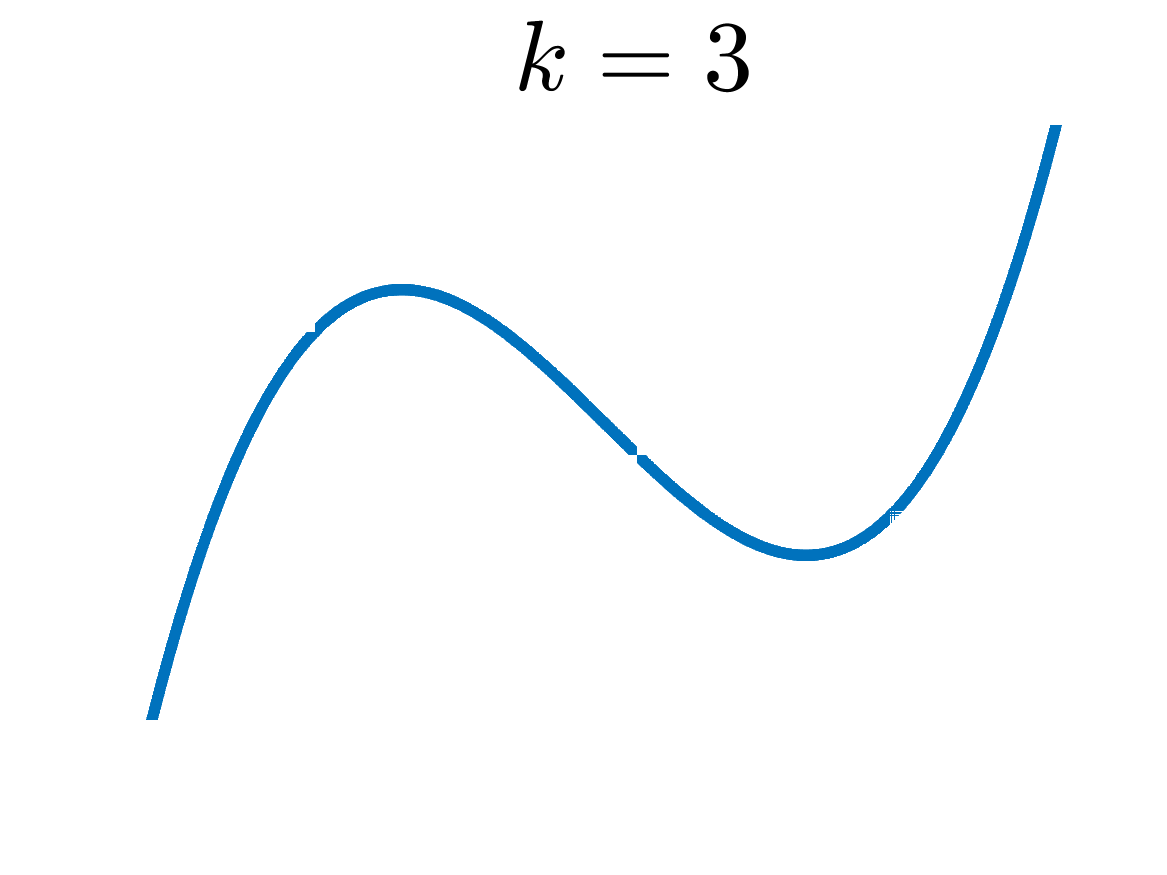
\includegraphics[width =0.18\textwidth]{ProgramsImages/Legendre_Degree_3_1D_k.png}  &
		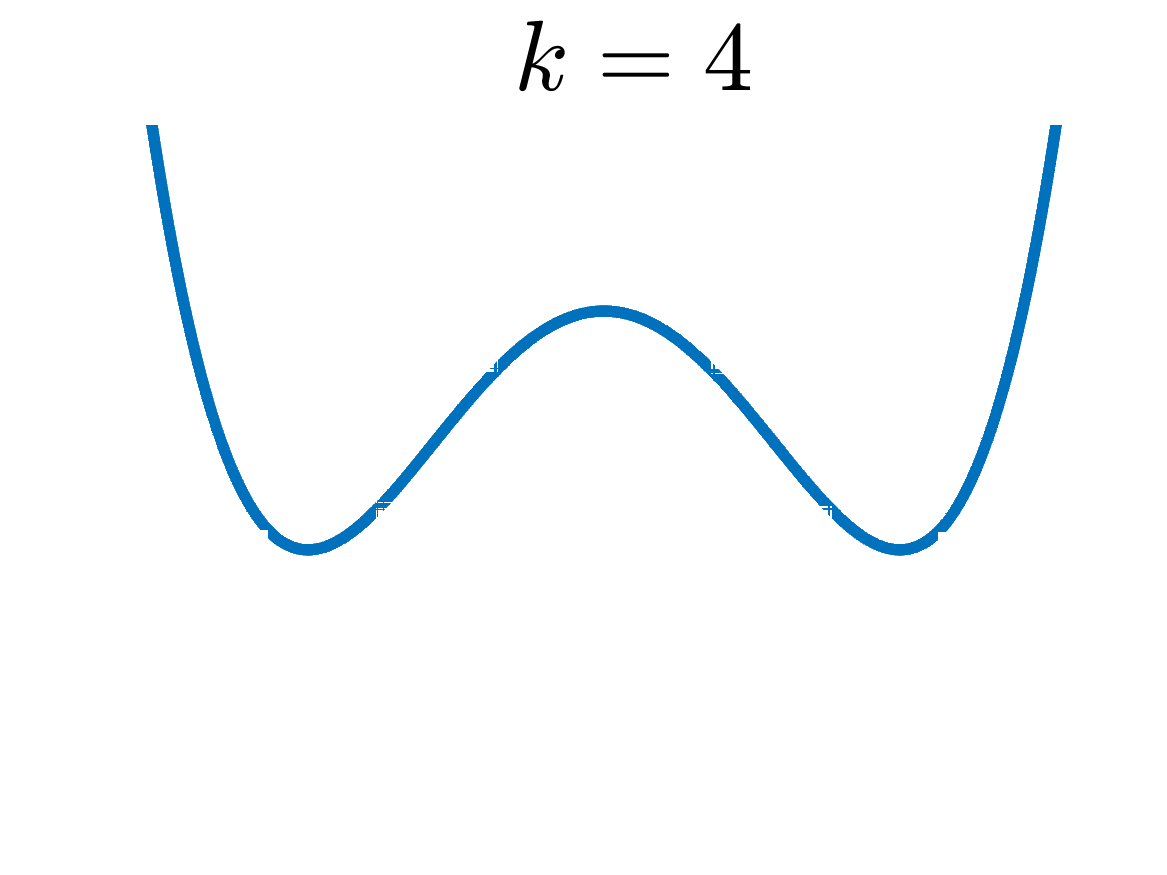
\includegraphics[width =0.18\textwidth]{ProgramsImages/Legendre_Degree_4_1D_k.png} 
	\tabularnewline[-7ex]
	Legendre
	\tabularnewline
\tabularnewline[2ex]
		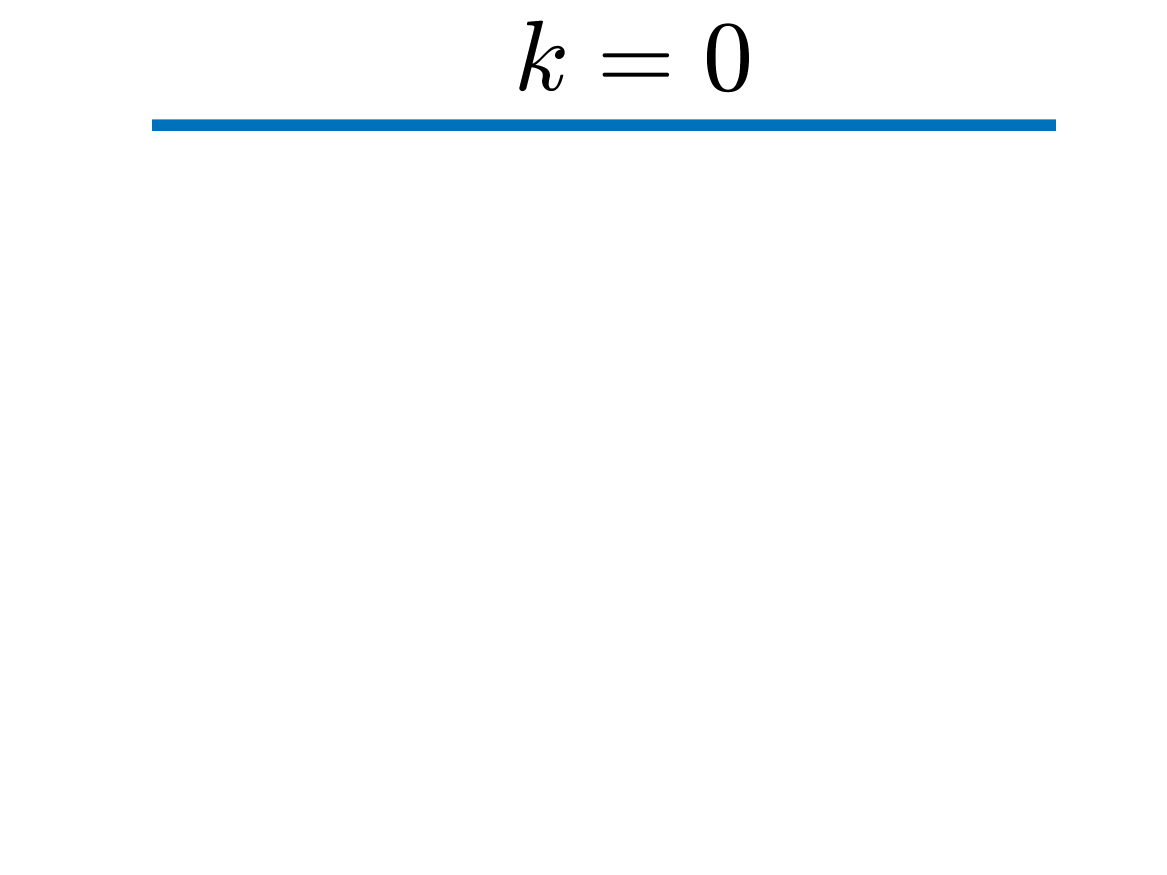
\includegraphics[width =0.18\textwidth]{ProgramsImages/Chebyshev_Degree_0_1D_k.png}  &
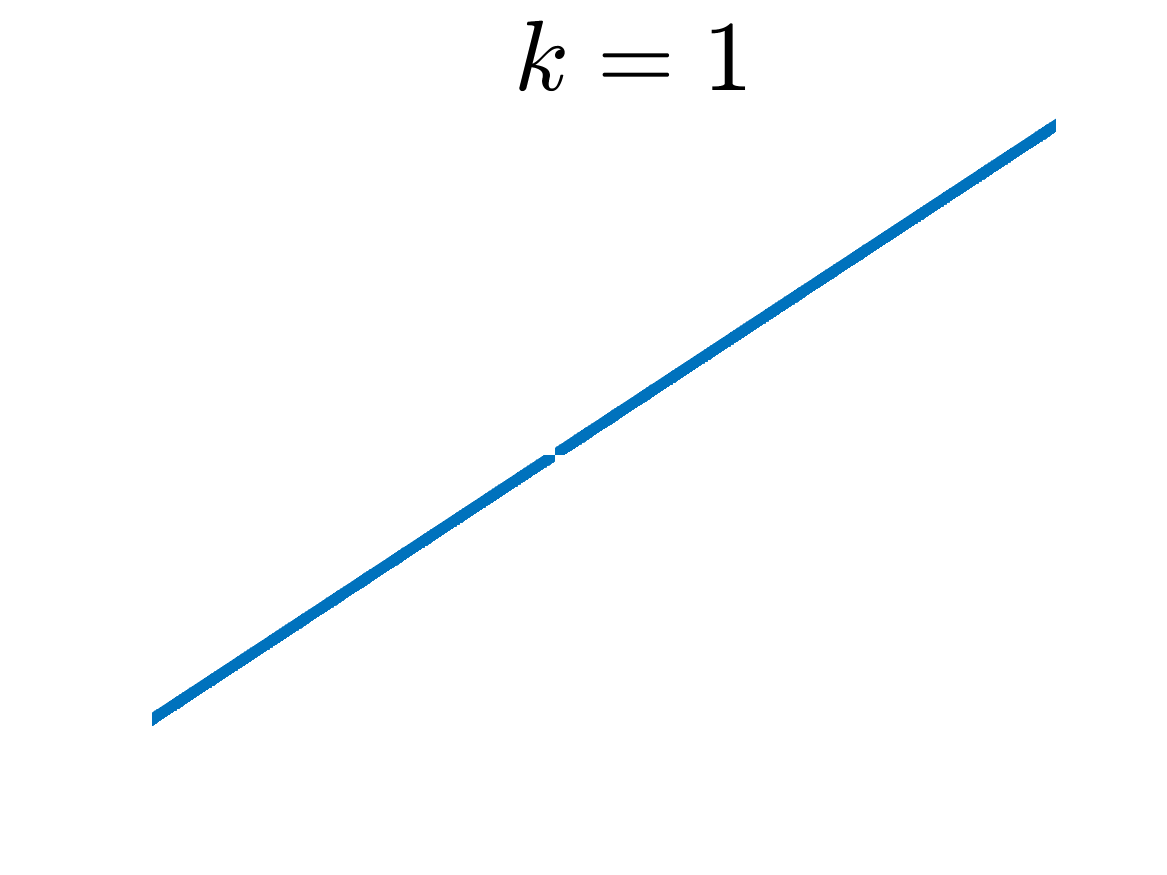
\includegraphics[width =0.18\textwidth]{ProgramsImages/Chebyshev_Degree_1_1D_k.png}  &
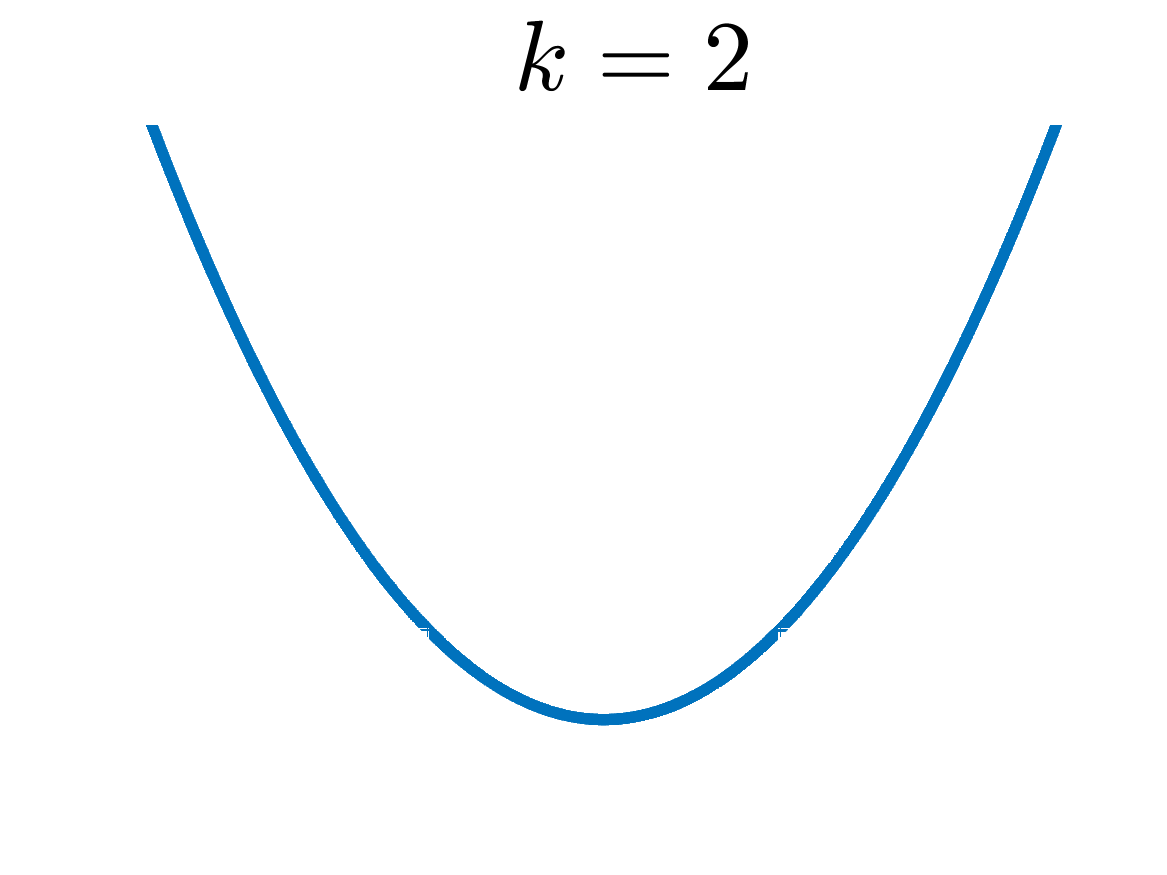
\includegraphics[width =0.18\textwidth]{ProgramsImages/Chebyshev_Degree_2_1D_k.png}  &
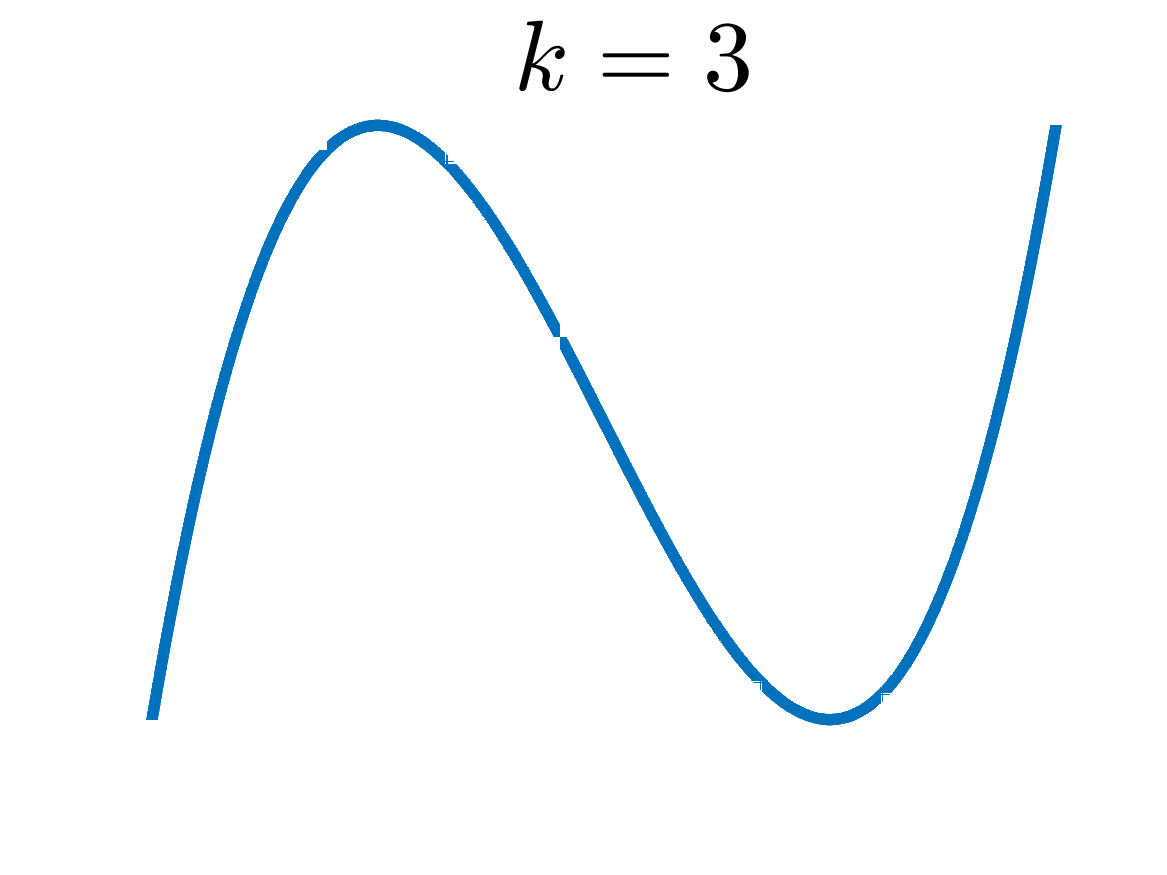
\includegraphics[width =0.18\textwidth]{ProgramsImages/Chebyshev_Degree_3_1D_k.png}  &
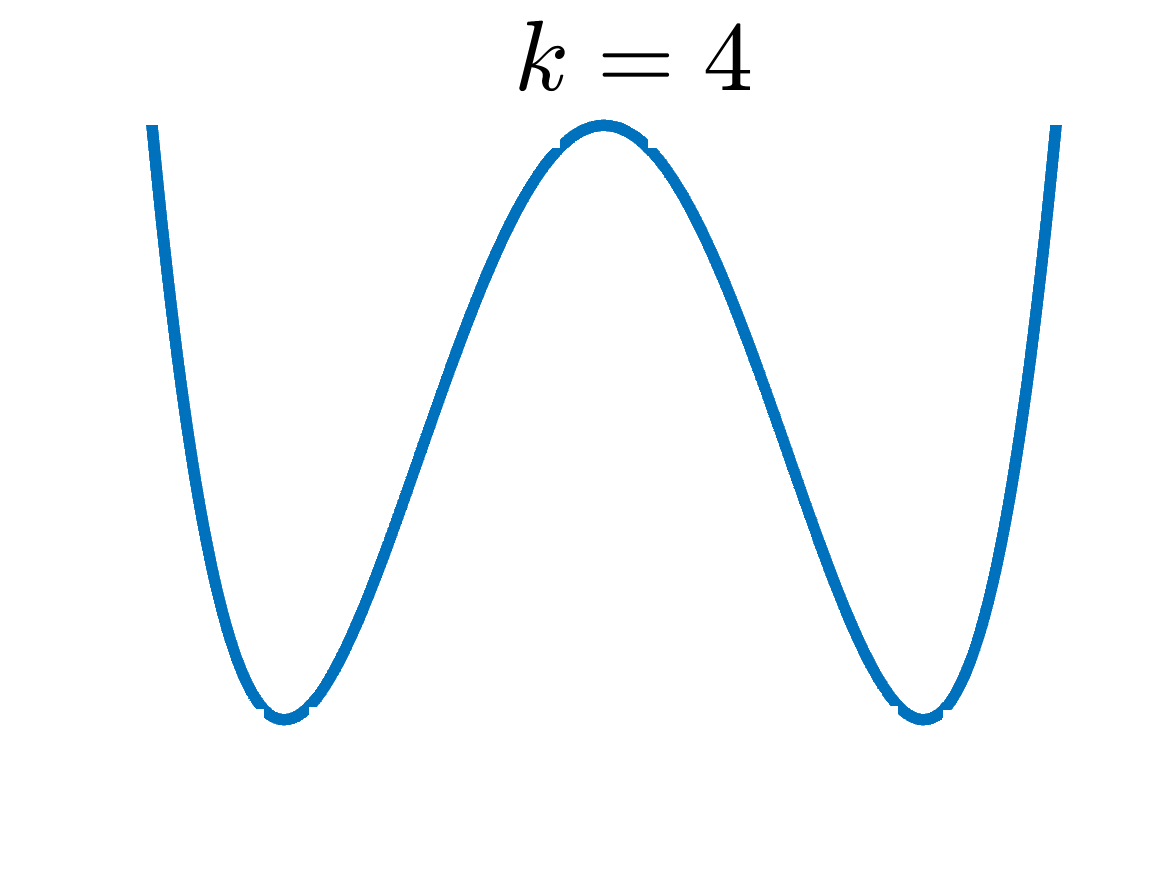
\includegraphics[width =0.18\textwidth]{ProgramsImages/Chebyshev_Degree_4_1D_k.png} 
\tabularnewline[-7ex]
Chebyshev
\tabularnewline
\tabularnewline[2ex]
		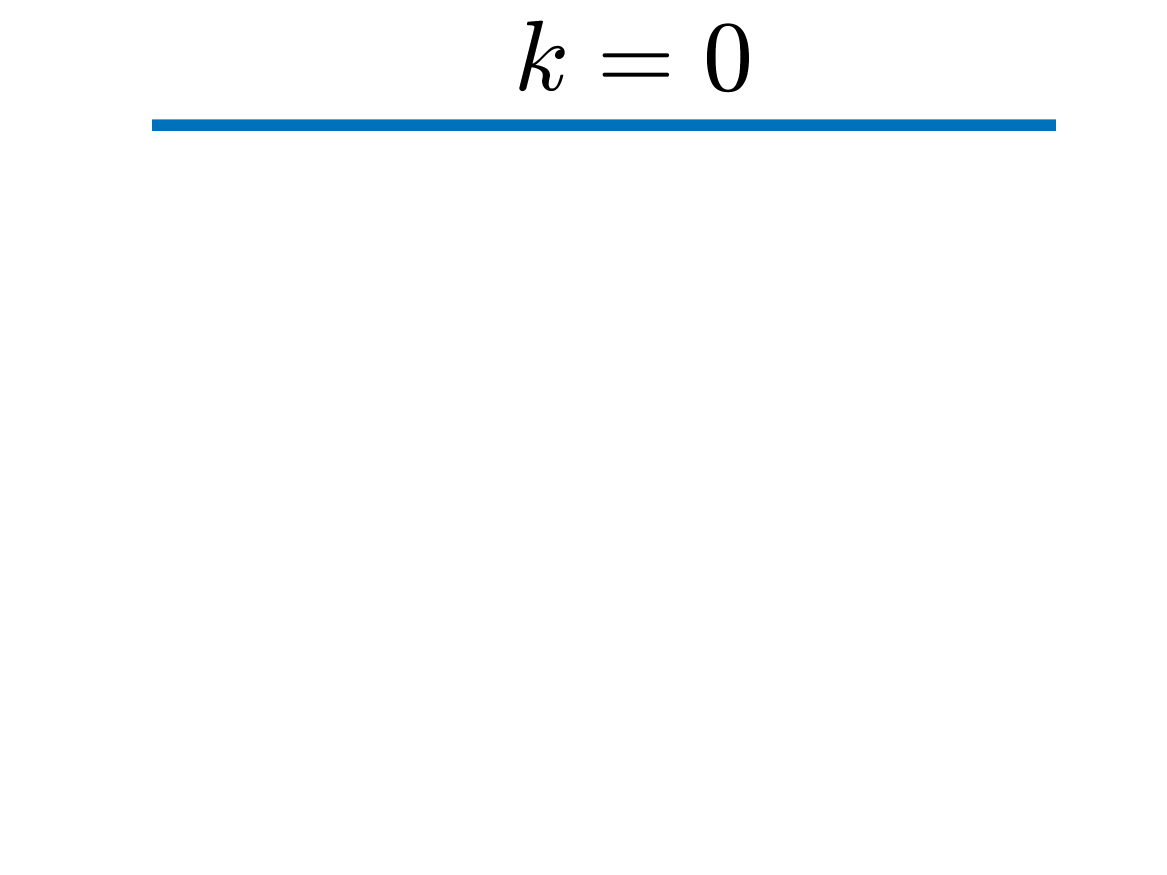
\includegraphics[width =0.18\textwidth]{ProgramsImages/Chebyshev_Degree_0_1D_k.png}  &
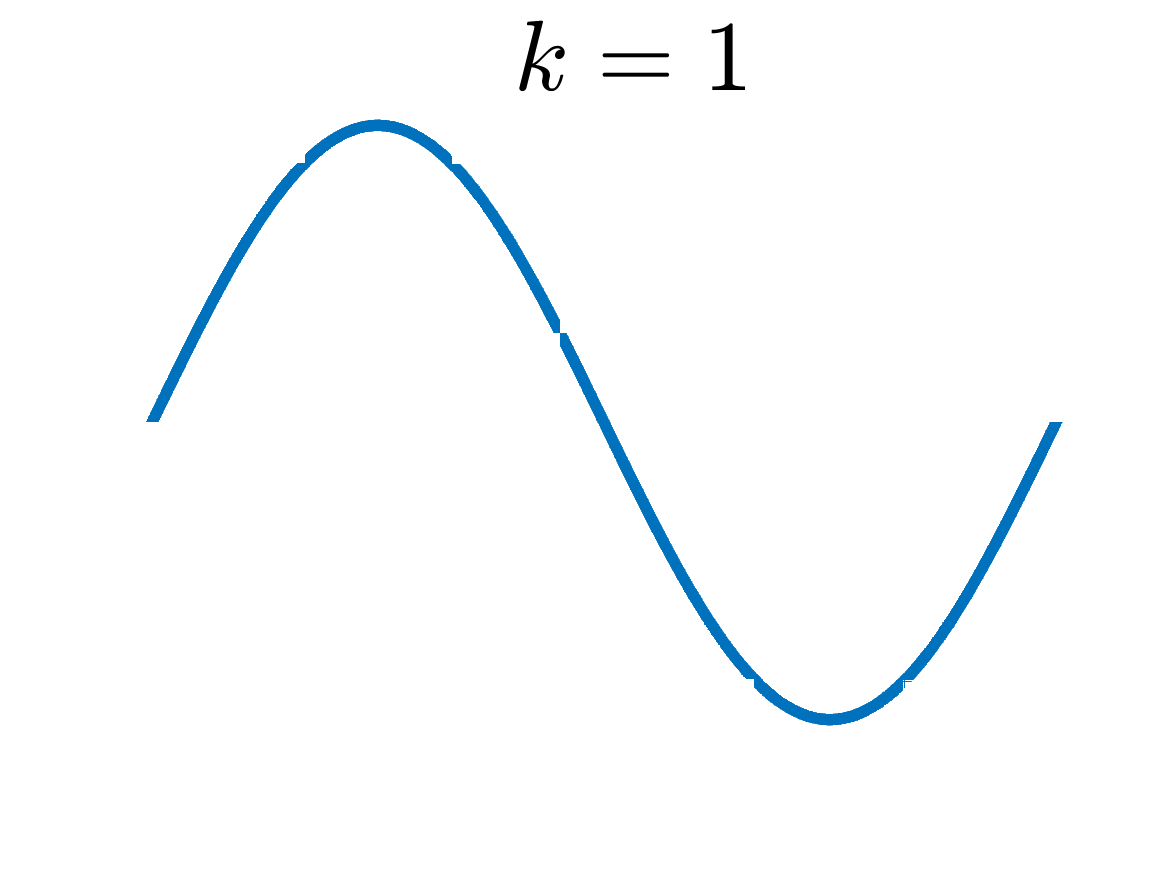
\includegraphics[width =0.18\textwidth]{ProgramsImages/CosineSine_Degree_1_1D_k.png}  &
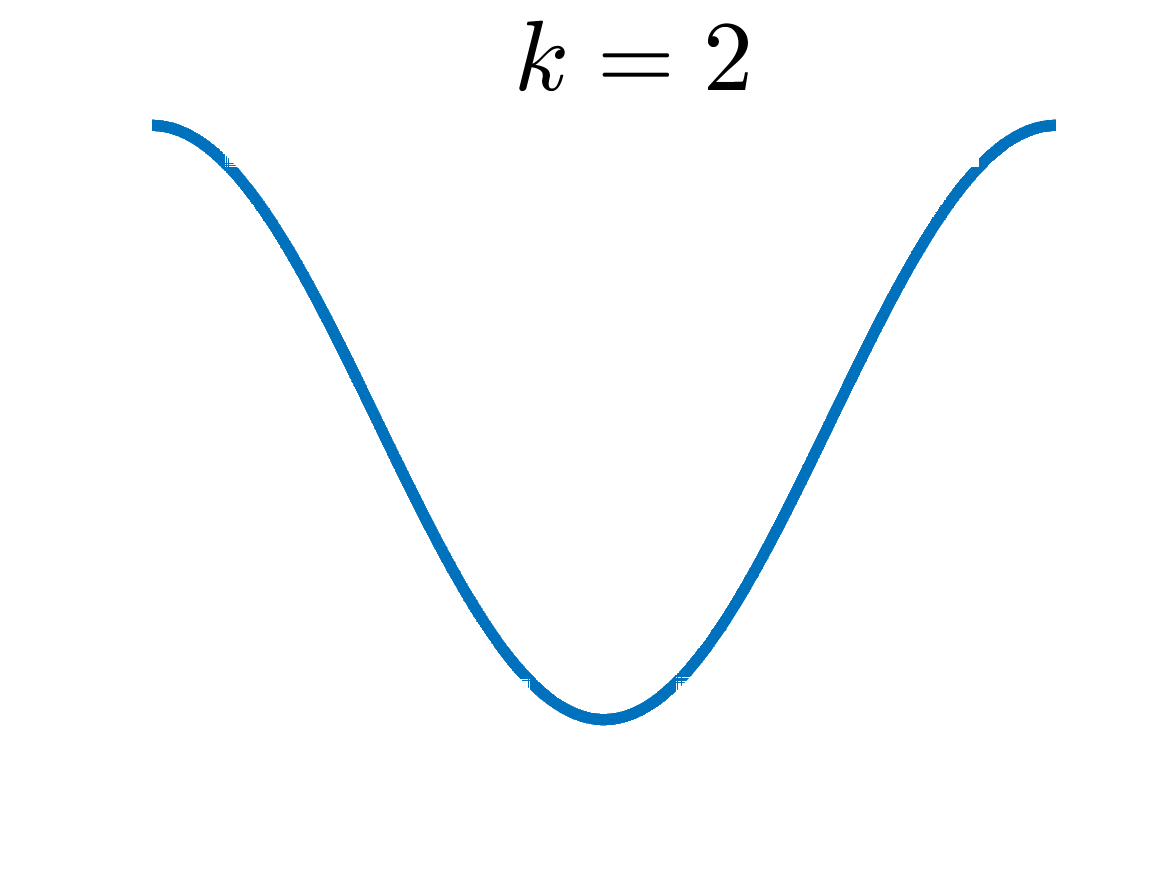
\includegraphics[width =0.18\textwidth]{ProgramsImages/CosineSine_Degree_2_1D_k.png}  &
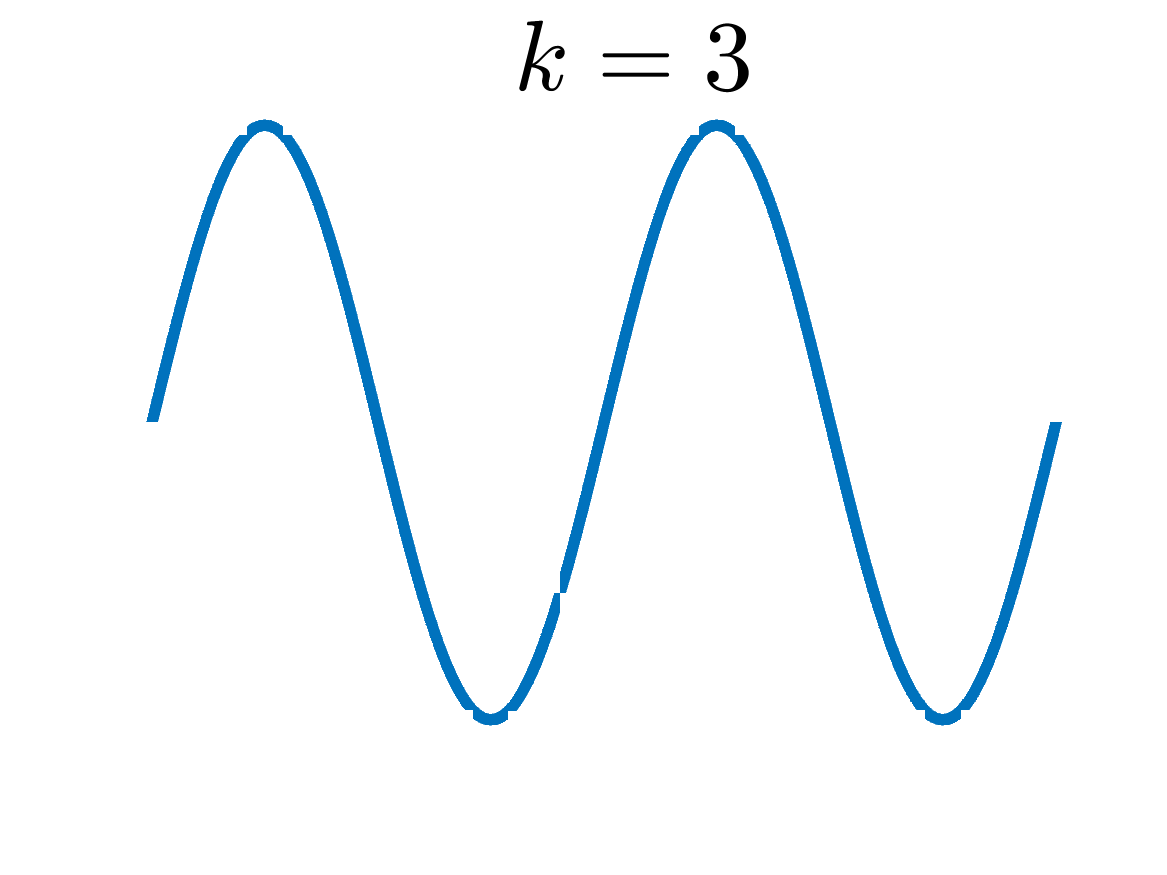
\includegraphics[width =0.18\textwidth]{ProgramsImages/CosineSine_Degree_3_1D_k.png}  &
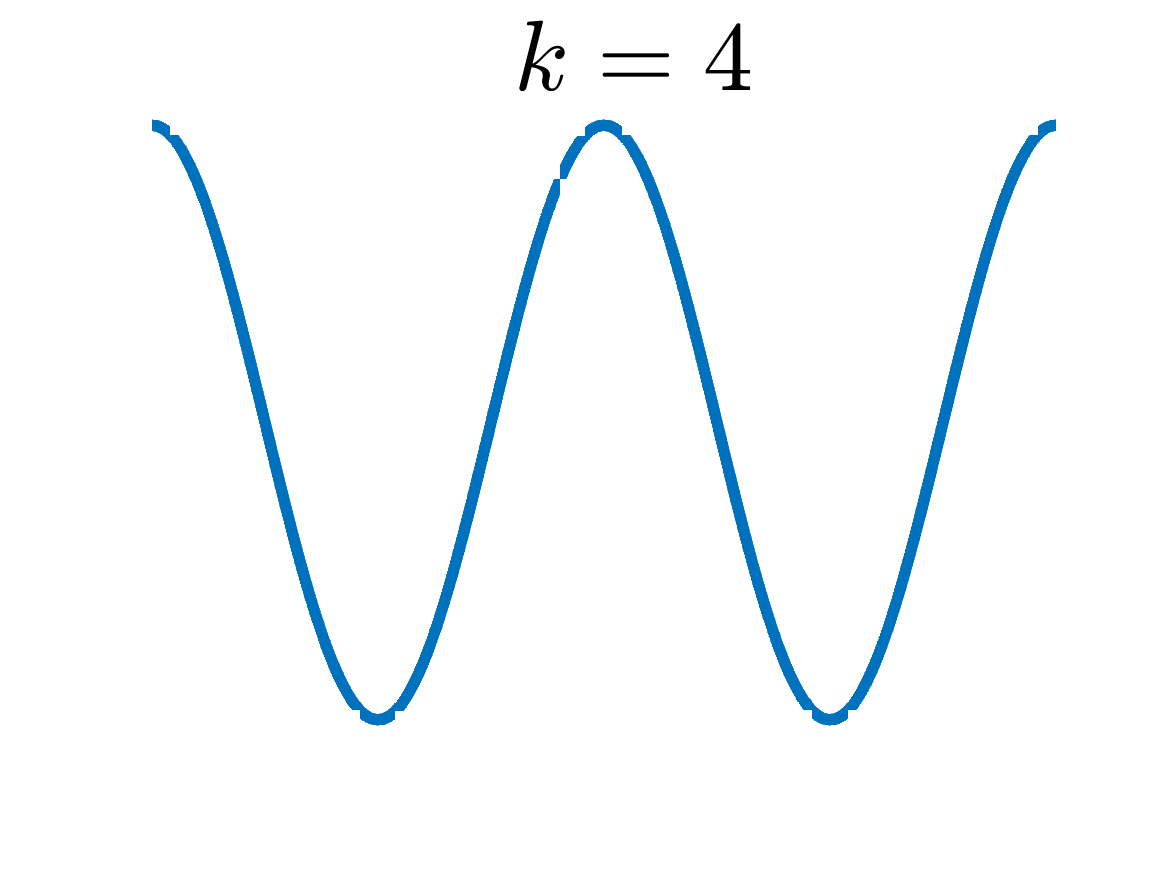
\includegraphics[width =0.18\textwidth]{ProgramsImages/CosineSine_Degree_4_1D_k.png} 
\tabularnewline[-7ex]
Sine and Cosine \tabularnewline
	\end{tabular}
\end{frame}

\againframe<2->{smoothness}

%%%%%%%%%%%%%%%%%%%%%%%%%%%%%%%%%%%%%%%%%%%%%%%%%%%%%%%%%%%%%%%%%%%%
\section{Tractability}
%%%%%%%%%%%%%%%%%%%%%%%%%%%%%%%%%%%%%%%%%%%%%%%%%%%%%%%%%%%%%%%%%%%%
\begin{frame}{Smoothness Cannot Save You from the Curse of Dimensionality\footfullcite{NovWoz08a}}
\vspace{-3ex}
For \alert{arbitrary $d$}, let $\{u_0 = 1, u_1\}$ be used to construct a product basis $\cf$ and $\cg$ (multlinear functions)

\vspace{-6ex}
\begin{gather*}
    \cf := \left \{ f(\vx) = \sum_{\vk \in \{0,1\}^d} \hf(\vk) u_\vk  : \norm[\cf]{f} : = \norm[2]{\left(\frac{\hf(\vk)}{\lambda_\vk} \right)_{\vk \in \{0,1\}^d} } < \infty \right \}, \qquad u_\vk(\vx) := \prod_{\ell = 1}^d u_{k_\ell} (x_\ell)\\
   \cg := \left \{ g = \sum_{\vk \in \{0,1\}^d} \hg(\vk) u_\vk  : \norm[\cg]{g} : = \norm[2]{\bigl(\hg(k) \bigr)_{\vk \in \{0,1\}^d} } < \infty \right \}, \qquad \lambda_\vk := \prod_{\ell = 1}^d \lambda^{k_\ell} = \lambda^{\norm[0]{\vk}}\\
   \app(f,n) = \sum_{i=1}^n \hf(\vk_i) u_{\vk_i} , \qquad 
   \lambda_{\vk_1} = 1 \ge \lambda = \lambda_{\vk_2} \ge \cdots \ge \lambda^{d}
   \uncover<2->{\\
    \alg(f,\varepsilon) 
    = \app(f,n^*), \quad n^* = \min\{n : \lambda_{\vk_{n+1}} \le R/\varepsilon\}, \qquad
    \norm[\cg]{f - \alg(f,\varepsilon)} \le \varepsilon \quad \forall f \in \cb_R\\ 
    \lambda_{\vk_n} = \Order\bigl(n^{-1/p}(1 + \lambda^p)^{\alert{d}/p}\bigr) \implies \COST(\cb_R,\varepsilon) = \Order\bigr(R^p\varepsilon^{-p}(1 + \lambda^p)^{\alert{d}/p} \bigl)} \quad \forall p
\end{gather*}


    
\end{frame}


\begin{frame}{Bases for Function Approximation}
\vspace{-3ex}
	\begin{tabular}{>{\centering}m{0.18\textwidth}>{\centering}m{0.18\textwidth}>{\centering}m{0.18\textwidth}>{\centering}m{0.18\textwidth}>{\centering}m{0.18\textwidth}}
		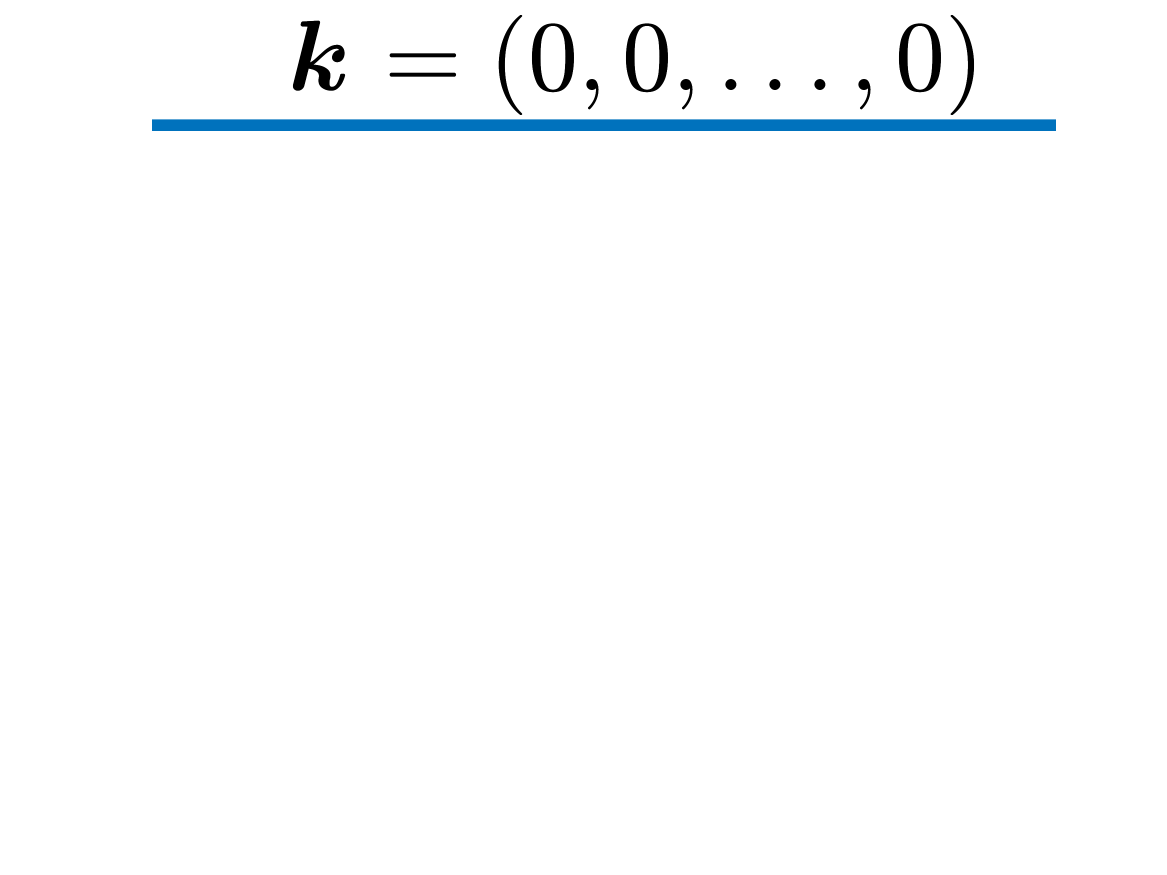
\includegraphics[width =0.18\textwidth]{ProgramsImages/Legendre_Degree_0_k.png}  &
		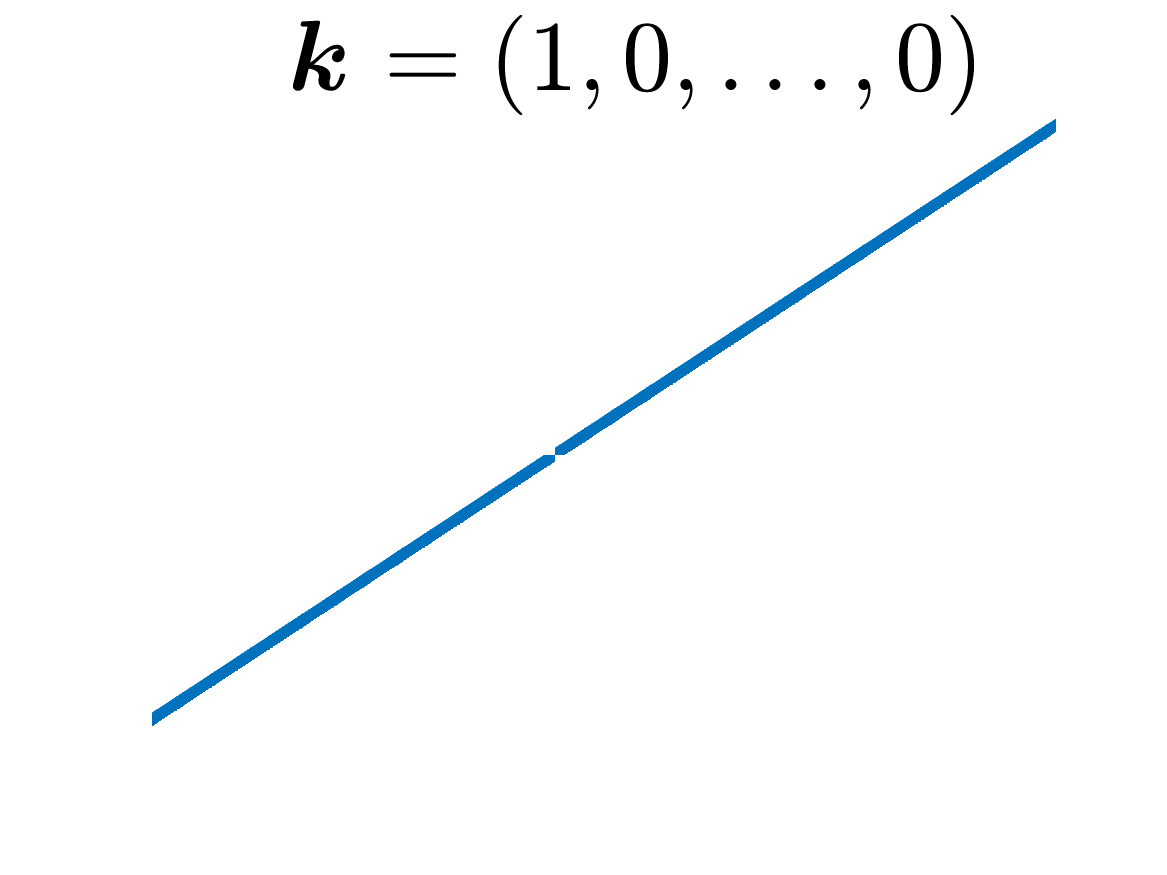
\includegraphics[width =0.18\textwidth]{ProgramsImages/Legendre_Degree_1_k.png}  &
		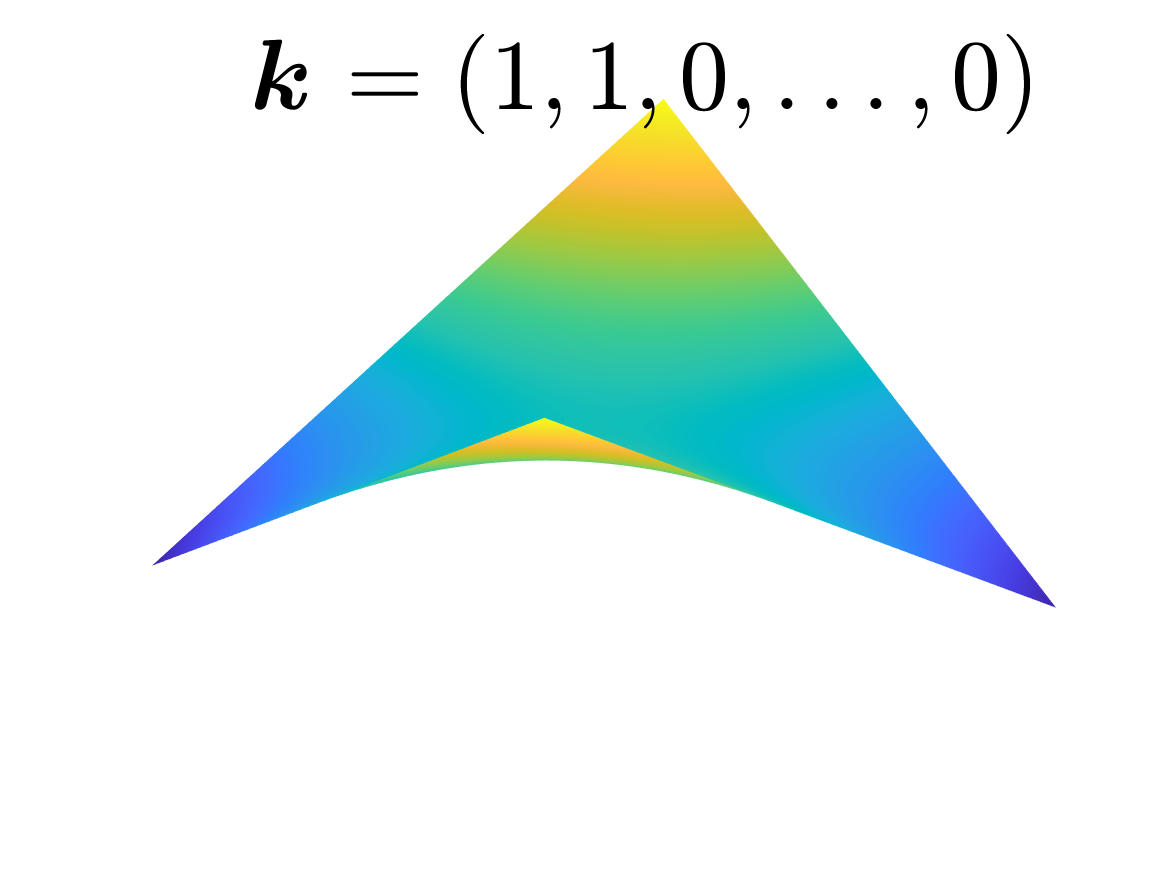
\includegraphics[width =0.18\textwidth]{ProgramsImages/Legendre_Degree_1_1_k.png}
		\tabularnewline[-7ex]
	Legendre
	\tabularnewline
\tabularnewline[2ex]
		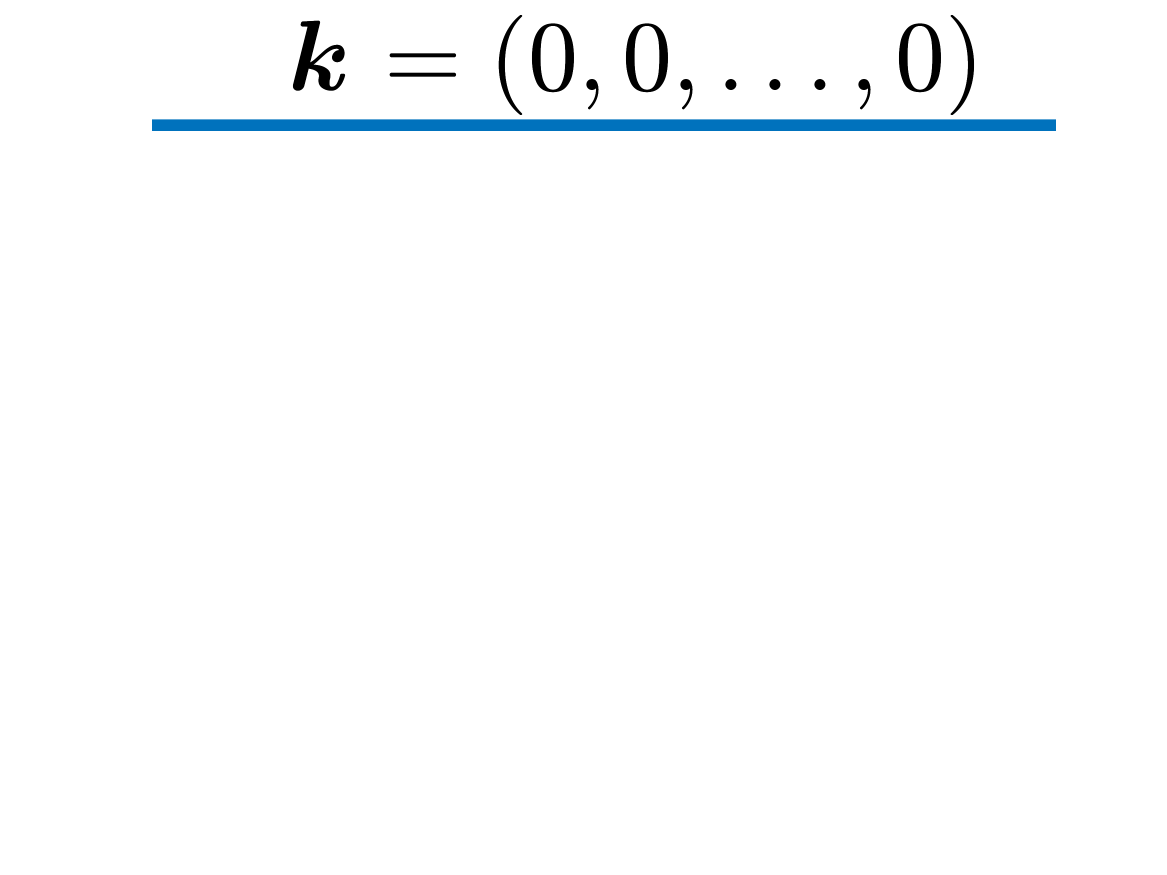
\includegraphics[width =0.18\textwidth]{ProgramsImages/Chebyshev_Degree_0_k.png}  &
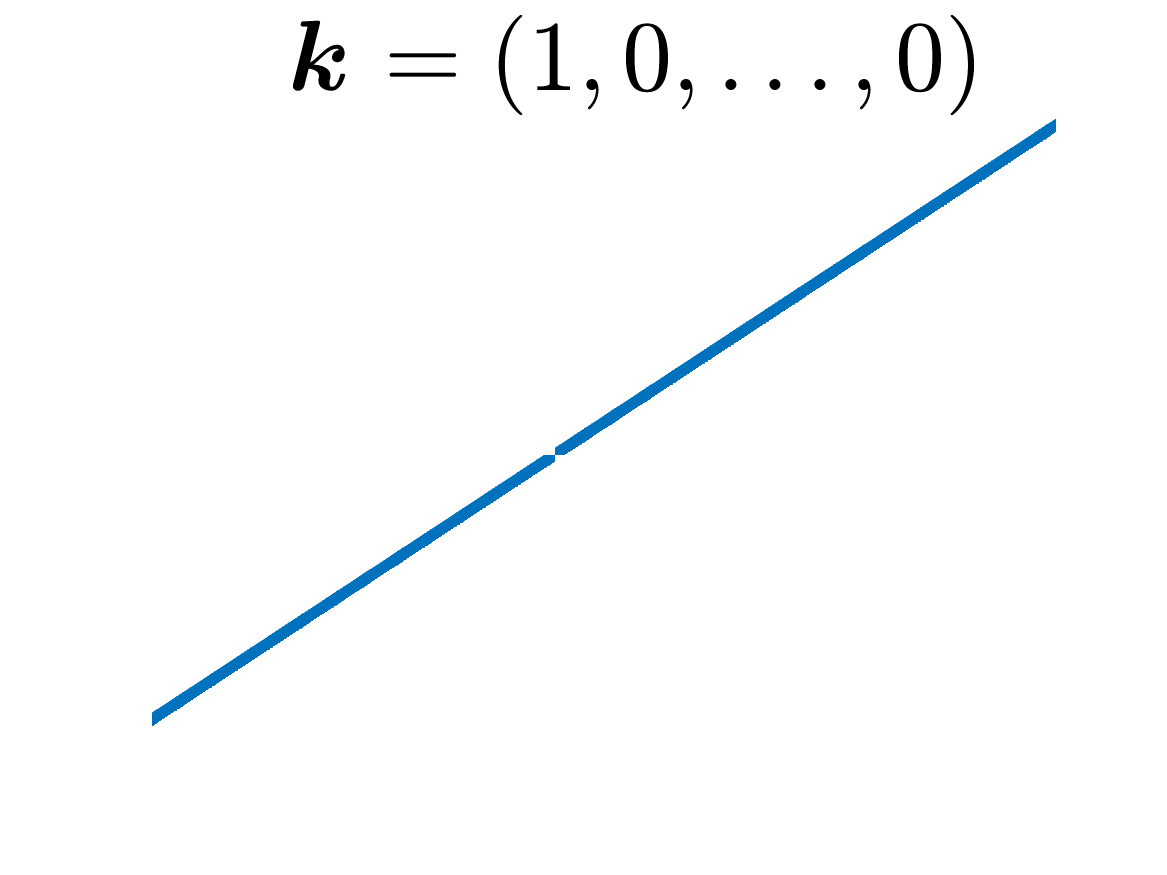
\includegraphics[width =0.18\textwidth]{ProgramsImages/Chebyshev_Degree_1_k.png}  &
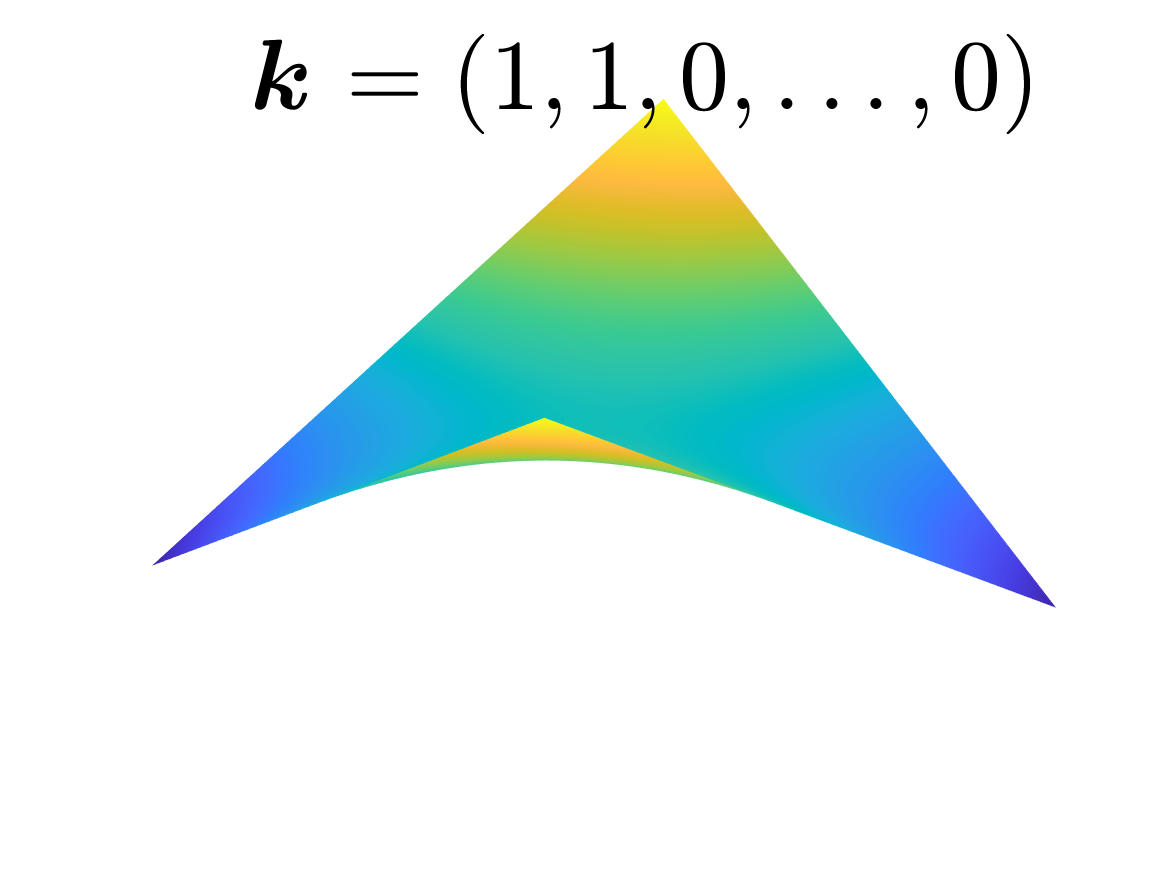
\includegraphics[width =0.18\textwidth]{ProgramsImages/Chebyshev_Degree_1_1_k.png}  
\tabularnewline[-7ex]
Chebyshev
\tabularnewline
\tabularnewline[2ex]
		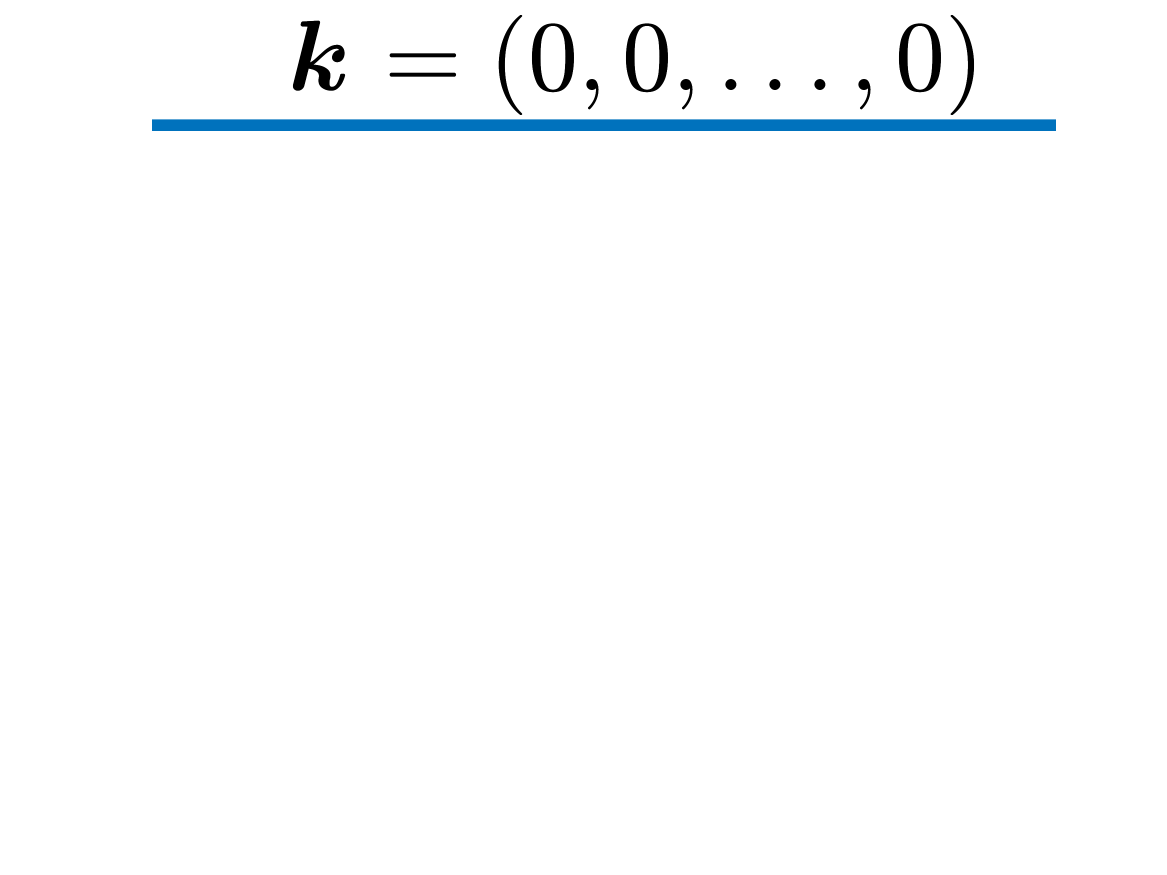
\includegraphics[width =0.18\textwidth]{ProgramsImages/Chebyshev_Degree_0_k.png}  &
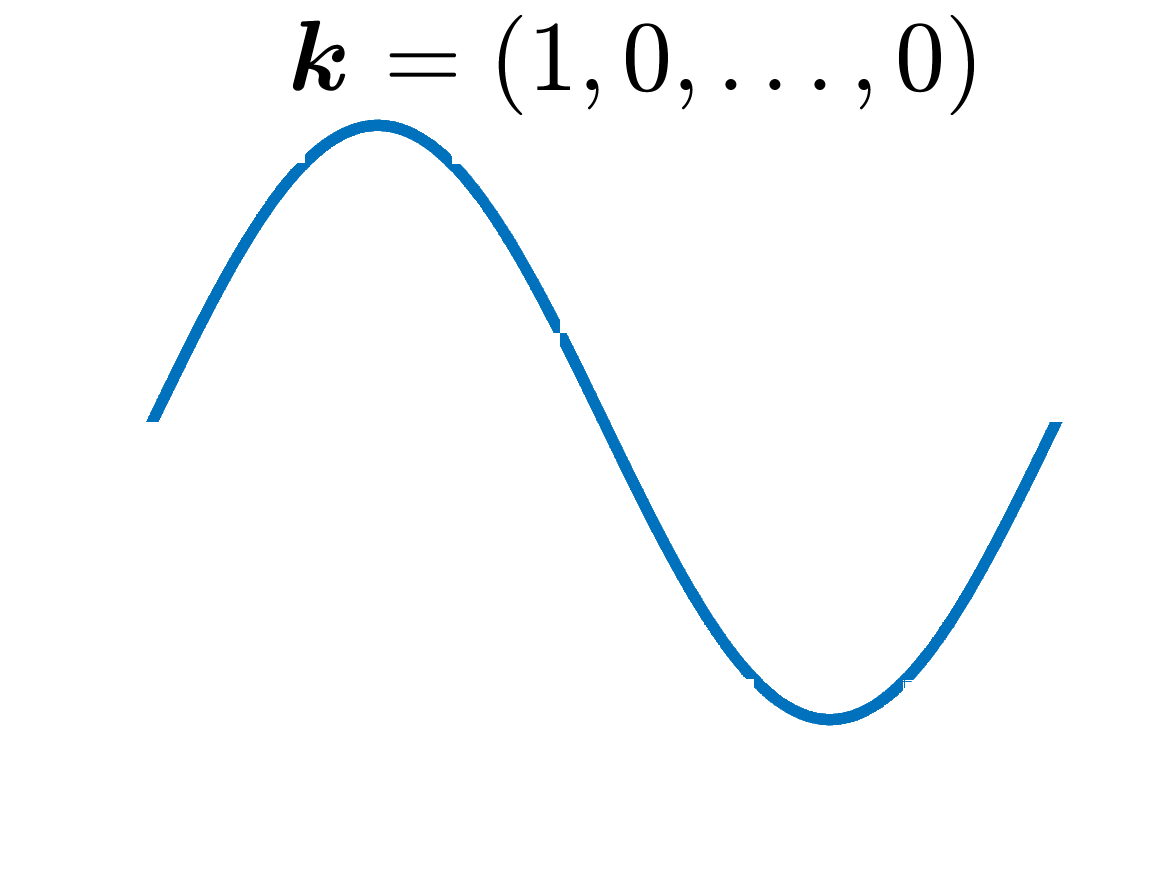
\includegraphics[width =0.18\textwidth]{ProgramsImages/CosineSine_Degree_1_k.png}  &
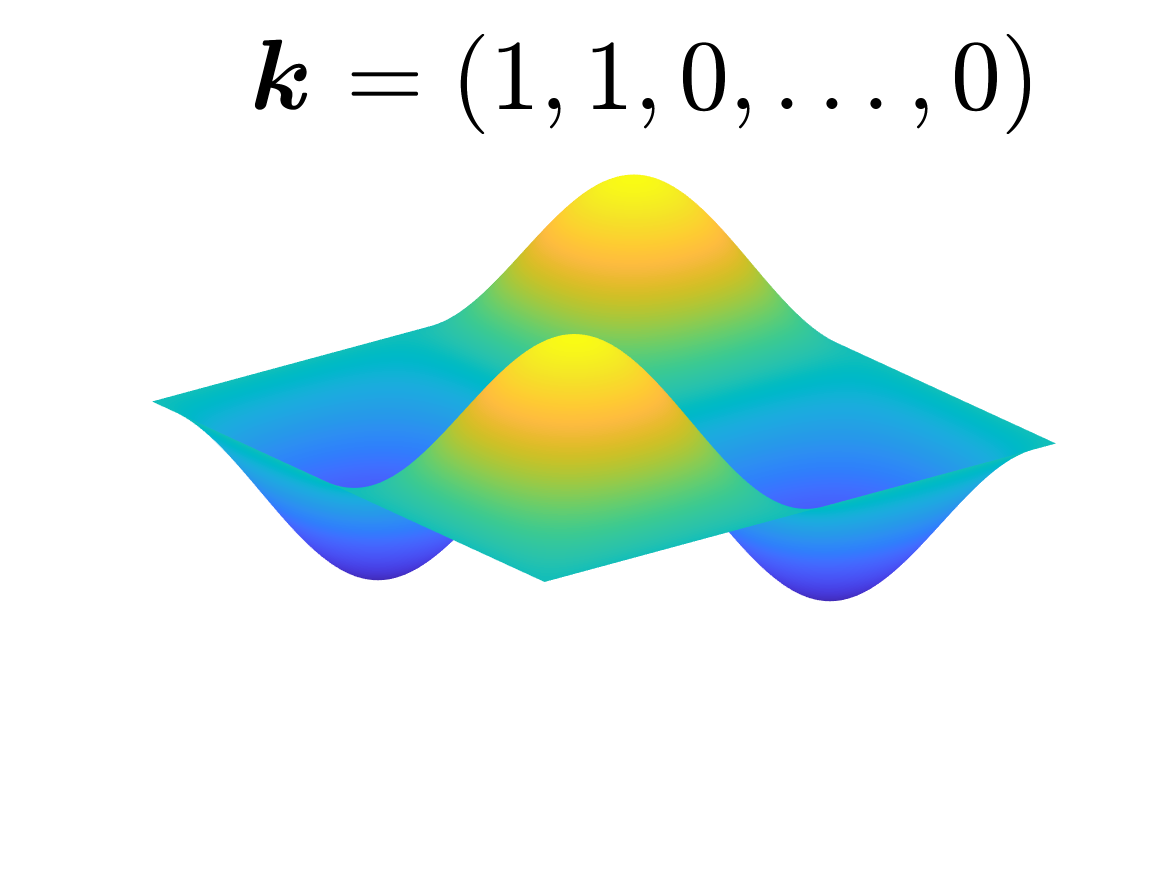
\includegraphics[width =0.18\textwidth]{ProgramsImages/CosineSine_Degree_1_1_k.png}   
\tabularnewline[-7ex]
Sine and Cosine \tabularnewline
	\end{tabular}
\end{frame}






\begin{frame}{Context}

\vspace{-5ex}

\begin{itemize}
    \item Given 
    \begin{description}[labelwidth = 8ex]
       \item[Black box] providing \only<1>{\alert{noisy} or }\alert{noiseless} information about $f$ \\
        e.g., function values, series coefficients, or linear functionals, \alert{costing} $\$(f)$ each
        
        \item[Error tolerance] $\varepsilon$
     
    \end{description}
    
    \item Want function $\alg(f,\varepsilon)$ \only<1>{(as a surrogate, for solving PDEs, for uncertainty quantification)} that is
    \begin{description}
        \item[Cheap] to evaluate
        
        \item[Accurate] $\norm[\cg]{f - \alg(f,\varepsilon)} \le \varepsilon$
        
        \item[Efficient] to construct

    \end{description}

	\item<2-> Fixed computation budget \alert{approximation} $\app(f,n) = \sum_{i=1}^n L_i(f) g_{i,n}$
	\begin{itemize}
	    \item $L_1(f), L_2(f), \ldots$ is input function information 
	    \item $\vg_n = (g_{1,n}, \ldots, g_{n,n}) \in \cg^n$
	    \item $ \alert{\COST(f,n)} = \Order(n \$(f) + \COST( \vg_n))$
	\end{itemize}
	
	\item<2-> \alert{Algorithm} $\alg(f,\varepsilon) = \app(f,n^*(f,\varepsilon))$ satisfying  
	$\norm[\cg]{f -  \app(f,n^*(f,\varepsilon))} \le \varepsilon$
		\begin{itemize}
	    \item $ \alert{\COST(f,\varepsilon)} = \COST(f,n^*(f,\varepsilon)) + \text{ cost to determine } n^*(f,\varepsilon)$
	\end{itemize}


\uncover<2->{\item \alert{Solvability:} what assumptions on $f$ to determine $n^*(f,\varepsilon) \in \naturals$ \alert{correctly}?  
	\only<3->{\smallscoop\only<4->{\hspace{-6ex}\raisebox{-1.5ex}{\color{red}\fontsize{40}{48}\selectfont $\times$}} or \smallcone}
\only<2>{
	
	\begin{itemize}
	\item $n^*(f,\varepsilon) = \min\{n : \norm[\cf \to \cg]{\sol - \app(\cdot,n)} \le \varepsilon / R\}$  if $f \in \smallscoop$ of radius $R$
	
	\item Alternative is to assume $f \in \smallcone$ and to bound $ \norm[\cf]{f}$ or equivalent\footfullcite{HicEtal17a,KunEtal19a,DinHic20a} \\
	\emph{What you do not see is not much worse than what you see?}
\end{itemize}}

\only<3->{\item \alert{Optimality:} is $n^*(f,\varepsilon)$ essentially as small as possible?
	
	\item \alert{Tractability:} does $n^*(f,\varepsilon)$ depend nicely on $d$?
}
}

\end{itemize}

\end{frame}

\end{document}

\begin{frame}{Solving General Linear Problems Using Series Coefficients\footfullcite{DinEtal20a}}
	
	\vspace{-7ex}
	
	\begin{align*}
	\only<1-2>{\cf &:= \left \{ f = \sum_{i=1}^\infty \hf(\vk_i) u_{\vk_i} : \norm[\cf]{f} := \norm[\rho]{\left(\frac{\bigabs{\hf(\vk_i)}}{\lambda_{\vk_i}} \right)_{i =1}^\infty} \right \} \qquad 
		\begin{minipage}{4.2cm}\raggedright  $\lambda_{\vk_1} \ge \lambda_{\vk_2} \ge \cdots > 0$ \\
		\alert{$\vlambda$ affects convergence rate \&  \\ tractability}\end{minipage}\\
		\cg &: = \biggl \{ g = \sum_{i=1}^\infty \hg(\vk_i) v_{\vk_i} : \norm[\cg]{g} := \bignorm[\tau]{\hg}\biggr \}, \qquad v_{\vk} = \sol(u_{\vk}) \\}
	\cc_{\vlambda, n_1, A} &: = \Biggl\{ f \in \cf : \norm[\cf]{f} \le A\norm[\rho]{\biggl ( \frac{\hf(\vk_i) }{\lambda_{\vk_i}} \biggr) _{i=1}^{n_1}} \Biggr\} \qquad 
		\begin{minipage}{4.2cm}\raggedright 
		\alert{what is observed initially \\ tells us enough}\end{minipage}  
		\uncover<2->{\\
	\app(f,n) &= \sum_{i=1}^{n} \hf(\vk_i) v_{\vk_i}\quad  \alert{\text{optimal for fixed }n}
	\qquad \norm[\cg]{\sol(f) - \app(f,n)} \le  \ERRN \\[-1ex]
\MoveEqLeft[4]{\ERRN := \underbrace{\left[ A^\rho \norm[\rho]{\left( \frac{\hf(\vk_i)}{\lambda_{\vk_i}} \right)_{i=1}^{n_1}}^\rho -  \norm[\rho]{\left(\frac{\hf(\vk_i)}{\lambda_{\vk_i}}\right)_{i=1}^n}^\rho \right]^{1/\rho}}_{\text{upper bound on } \norm[\cf]{f - \sum_{i=1}^{n} \hf(\vk_i) u_{\vk_i}}}
\, \underbrace{\bignorm[\rho']{\bigl( \lambda_{\vk_i}  \bigr)_{i = n+1}^{\infty}}}_{\norm[\cf \to \cg]{\sol - \app(\cdot,n)}}  
\quad \begin{minipage}{2cm}
$\displaystyle \frac 1\rho + \frac 1 {\rho'} = \frac 1 \tau $\\[1ex]
\alert{\text{data-driven}}
\end{minipage}
}
}
    \only<3->{\\[-1ex]
	\alert{A(f,\varepsilon)} & \alert{= \Sapp(f,n_k)} \text{ for the smallest $k$ satisfying } \alert{\sigma_k(f) \le \frac{\varepsilon \sqrt{1 - b^2}}{ab}}
	\\ 
		\MoveEqLeft{\alert{\COST(A,\cc,\varepsilon,\rho) = n_{\ell^\dagger}}, \quad 
			\ell^\dagger \le \min \left \{\ell \in \naturals : \frac{\rho^2}{\varepsilon^2} \le \frac{(1 - b^2)}{a^2b^2} \left[ \sum_{k=1}^{\ell-1} \frac{b^{2(k-\ell)}}{a^2\lambda_{n_{k-1}+1}^2} + \frac{1}{\lambda_{n_{\ell-1}+1}^2}\right]   \right\}} \\
		\MoveEqLeft{\COST(A,\cc,\varepsilon,\rho) \text{ \alert{essentially no worse than} } \comp(\ca(\cc,\LambdaAll),\varepsilon,\rho)}\\
		\MoveEqLeft{\text{\alert{No} tractability results}}}
	\end{align*}
	
\end{frame}

\begin{frame}{Multivariate Linear Problems}
\vspace{-3ex}
\begin{tabular}{p{0.47\textwidth}p{0.5\textwidth}}
Given $f \in \cf$ find $S(f) \in \cg$, where \\
$\sol: \cf \to \cg$ is linear, e.g., 
\begin{gather*}
    S(f) = \int_{\reals^d} f(\vx) \, \varrho(\vx) \, \dif \vx\\
    S(f) = f\\
    S(f) = \frac{\partial f}{\partial x_1} \\
    - \nabla^2 S(f) = f, \ \  S(f) = 0 \text{ on boundary}
\end{gather*}
&
\vspace{-7ex}
\alert{Successful algorithms}
\vspace{-3ex}
\begin{multline*}
    \ca(\cc,\Lambda) : = \{\app: \cc \times (0,\infty) \to \cg \text{ such that } \\
\norm[\cg]{\sol(f) - \app(f,\varepsilon) } \le \varepsilon \ \ \forall f \in \cc \subseteq \cf, \ \varepsilon > 0 \}
\end{multline*}

\vspace{-1ex}
where $\app(f,\varepsilon)$ depends on \alert{function values}, $\LambdaStd$, \alert{Fourier coefficients}, $\LambdaSer$, or \alert{any linear functionals}, $\LambdaAll$, e.g., 

\vspace{-4ex}
\begin{gather*}
    \Sapp(f,n) = \sum_{i=1}^n f(\vx_i) \, g_i, \quad g_i \in \cg \\
    \Sapp(f,n) = \sum_{i=1}^n \hf_i \, g_i, \quad g_i \in \cg \\
    \Sapp(f,n) = \sum_{i=1}^n L_i(f) \, g_i, \quad g_i \in \cg \\
\end{gather*}

\vspace{-5ex}
\hfill \hfill \alert{$\app(f,\varepsilon) = \Sapp(f,n) + $ stopping criterion}\newline
\phantom{a} \hfill \hfill \alert{$\cc$ is a \smallcone}

\end{tabular}
    
\end{frame}

\begin{frame}{Issues}

\vspace{-3ex}

\begin{tabular}{p{0.47\textwidth}p{0.5\textwidth}}
Given $f \in \cf$ find $S(f) \in \cg$, where \\
$\sol: \cf \to \cg$ is linear

\bigskip

\alert{Successful algorithms}
\vspace{-2ex}
\begin{multline*}
    \ca(\cc,\Lambda) : = \{\app: \cc \times (0,\infty) \to \cg \text{ such that } \\
\norm[\cg]{\sol(f) - \app(f,\varepsilon) } \le \varepsilon \ \ \forall f \in \cc \subseteq \cf, \ \varepsilon > 0 \}
\end{multline*}

\vspace{-1ex}
where $\app(f,\varepsilon)$ depends on \alert{function values}, $\LambdaStd$, \alert{Fourier coefficients}, $\LambdaSer$, or \alert{any linear functionals}, $\LambdaAll$
&

\vspace{-9ex}
\uncover<1->{\alert{Solvability}\footfullcite{KunEtal19a}: $\ca(\cc,\Lambda) \ne \emptyset$

\smallskip

\alert{Construction}: Find $\app \in \ca(\cc,\Lambda)$}

\smallskip

\uncover<2->{\alert{Cost}: $\COST(\app,f,\varepsilon) = $ \# of function data
\newline
 $\COST(\app,\cc,\varepsilon, \rho) = \max_{f \in \cc \cap \cb_{\rho}} \COST(\app,f,\varepsilon)$
 \newline
 $\cb_{\rho} := \{f \in \cf : \norm[\cf]{f} \le \rho \}$
 
 \smallskip

\alert{Complexity}\footfullcite{TraWasWoz88}: $\comp(\ca(\cc,\Lambda),\varepsilon,\rho)$ 
\newline \phantom{a} \hfill \hfill $= \min_{\app \in \ca(\cc,\Lambda)} \COST(\app,\cc,\varepsilon, \rho)$

\alert{Optimality}:  \newline \phantom{a} \hfill \hfill $\COST(\app,\cc,\varepsilon, \rho) \le \comp(\ca(\cc,\Lambda),\alert{\omega} \varepsilon,\rho)$}

\smallskip

\uncover<3->{\alert{Tractability}\footfullcite{NovWoz08a}: $\comp(\ca(\cc,\Lambda),\varepsilon, \rho) \le C \rho^p\varepsilon^{-p} d^{q} $}

\smallskip
\uncover<4->{\alert{Implementation} in open source software}

\vspace{-6ex}

\phantom{a}

\end{tabular}

    
\end{frame}


\finalthanksnote{These slides are  available at \\  \href{https://speakerdeck.com/fjhickernell/ricam-2018-nov}{\nolinkurl{speakerdeck.com/fjhickernell/ricam-2018-nov}}}


\thankyouframe

\begin{frame}[allowframebreaks]
	\frametitle{References}
\printbibliography
\end{frame}


\begin{frame}
	\frametitle{An Alternative Cone Like Our Cone}
	\vspace{-5.5ex}
	\begin{equation*}
	\norm[\cf]{f} : = \norm[\rho]{\biggl ( \frac{\hf(\vk_i) }{\lambda_{\vk_i}} \biggr) _{i=1}^\infty}, \quad \lambda_{\vk_i} \downarrow 0, \qquad
	\norm[\cf']{f} : = \norm[\rho]{\biggl ( \frac{\hf(\vk_i) \omega_i}{\lambda_{\vk_i}} \biggr) _{i=1}^\infty},  
	\quad \omega_{i} \downarrow
		\end{equation*}
		\vspace{-2ex}
		\begin{multline*}
	\{ f \in \cf : \norm[\cf]{f} \le A'\norm[\cf']{f}\} 
	=: 	\alert{\cc'_{\vlambda, \vomega, A'} \subseteq \cc_{\vlambda, n_1, A}} : = \biggl\{ f \in \cf : \norm[\cf]{f} \le A\norm[\rho]{\biggl ( \frac{\hf(\vk_i) }{\lambda_{\vk_i}} \biggr) _{i=1}^{n_1}} \biggr\} \\
\text{for } A \ge \omega_1A'\left[\frac{1 + (\omega_{n_1+1}/\omega_1)^\rho}{1 - (\omega_{n_1+1}A')^\rho}\right]^{1/\rho}, \ \ \omega_{n_1+1}A' < 1 
		\end{multline*}

\only<1>{\vspace{-6ex}} 
	For any $f \in 	\cc'_{A'} $ it follows that 
	\begin{align*}
\only<1>{\norm[\cf']{f}^\rho- \norm[\rho]{\biggl ( \frac{\hf(\vk_i) \omega_i }{\lambda_{\vk_i}} \biggr) _{i=1}^{n_1}}^\rho 
	& = \norm[\rho]{\biggl ( \frac{\hf(\vk_i) \omega_i }{\lambda_{\vk_i}} \biggr) _{i=n_1 + 1}^{\infty}}^\rho \\
    & \le \omega_{n_1+1}^\rho \norm[\rho]{\biggl ( \frac{\hf(\vk_i) }{\lambda_{\vk_i}} \biggr) _{i=n_1 + 1}^{\infty}}^\rho 
     = \omega_{n_1+1}^\rho \left[ \norm[\cf]{f}^\rho - \norm[\rho]{\biggl ( \frac{\hf(\vk_i) }{\lambda_{\vk_i}} \biggr) _{i=1}^{n_1}}^\rho \right ]\\	
     & \le \omega_{n_1+1}^\rho \left[ A'{}^\rho \norm[\cf']{f}^\rho - \omega_1^{-\rho} \norm[\rho]{\biggl ( \frac{\hf(\vk_i) \omega_i}{\lambda_{\vk_i}} \biggr) _{i=1}^{n_1}}^\rho \right ]}
 \only<2>{
 	\norm[\cf']{f}^\rho & \le \frac{1 + (\omega_{n_1+1}/\omega_1)^\rho}{1 - (\omega_{n_1+1}A')^\rho} \norm[\rho]{\biggl ( \frac{\hf(\vk_i) \omega_i }{\lambda_{\vk_i}} \biggr) _{i=1}^{n_1}}^\rho \\
  	\norm[\cf]{f} & \le \omega_1A'\left[\frac{1 + (\omega_{n_1+1}/\omega_1)^\rho}{1 - (\omega_{n_1+1}A')^\rho}\right]^{1/\rho} \norm[\rho]{\biggl ( \frac{\hf(\vk_i)}{\lambda_{\vk_i}} \biggr) _{i=1}^{n_1}}
}
	\end{align*}
\end{frame}

\begin{frame}
	\frametitle{An Alternative Cone Like Our Cone}
	\vspace{-5.5ex}
	\begin{equation*}
	\norm[\cf]{f} : = \norm[\rho]{\biggl ( \frac{\hf(\vk_i) }{\lambda_{\vk_i}} \biggr) _{i=1}^\infty}, \quad \lambda_{\vk_i} \downarrow 0, \qquad
	\norm[\cf']{f} : = \norm[\rho]{\biggl ( \frac{\hf(\vk_i) \omega_i}{\lambda_{\vk_i}} \biggr) _{i=1}^\infty},  
	\quad \omega_{i} \downarrow
		\end{equation*}
		\vspace{-2ex}
		\begin{multline*}
	\{ f \in \cf : \norm[\cf]{f} \le A'\norm[\cf']{f}\} 
	=: 	\alert{\cc'_{\vlambda, \vomega, A'} \supseteq \cc_{\vlambda, n_1, A}} : = \biggl\{ f \in \cf : \norm[\cf]{f} \le A\norm[\rho]{\biggl ( \frac{\hf(\vk_i) }{\lambda_{\vk_i}} \biggr) _{i=1}^{n_1}} \biggr\} \\
\text{for } A = \omega_1A'\left[\frac{1 + (\omega_{n_1+1}/\omega_1)^\rho}{1 - (\omega_{n_1+1}A')^\rho}\right]^{1/\rho}, \ \ \omega_{n_1+1}A' < 1 
		\end{multline*}

\only<1>{\vspace{-6ex}} 
	For any $f \in 	\cc'_{A'} $ it follows that 
	\begin{align*}
\only<1>{\norm[\cf']{f}^\rho- \norm[\rho]{\biggl ( \frac{\hf(\vk_i) \omega_i }{\lambda_{\vk_i}} \biggr) _{i=1}^{n_1}}^\rho 
	& = \norm[\rho]{\biggl ( \frac{\hf(\vk_i) \omega_i }{\lambda_{\vk_i}} \biggr) _{i=n_1 + 1}^{\infty}}^\rho \\
    & \le \omega_{n_1+1}^\rho \norm[\rho]{\biggl ( \frac{\hf(\vk_i) }{\lambda_{\vk_i}} \biggr) _{i=n_1 + 1}^{\infty}}^\rho 
     = \omega_{n_1+1}^\rho \left[ \norm[\cf]{f}^\rho - \norm[\rho]{\biggl ( \frac{\hf(\vk_i) }{\lambda_{\vk_i}} \biggr) _{i=1}^{n_1}}^\rho \right ]\\	
     & \le \omega_{n_1+1}^\rho \left[ A'{}^\rho \norm[\cf']{f}^\rho - \omega_1^{-\rho} \norm[\rho]{\biggl ( \frac{\hf(\vk_i) \omega_i}{\lambda_{\vk_i}} \biggr) _{i=1}^{n_1}}^\rho \right ]}
 \only<2>{
 	\norm[\cf']{f}^\rho & \le \frac{1 + (\omega_{n_1+1}/\omega_1)^\rho}{1 - (\omega_{n_1+1}A')^\rho} \norm[\rho]{\biggl ( \frac{\hf(\vk_i) \omega_i }{\lambda_{\vk_i}} \biggr) _{i=1}^{n_1}}^\rho \\
  	\norm[\cf]{f} & \le \omega_1A'\left[\frac{1 + (\omega_{n_1+1}/\omega_1)^\rho}{1 - (\omega_{n_1+1}A')^\rho}\right]^{1/\rho} \norm[\rho]{\biggl ( \frac{\hf(\vk_i)}{\lambda_{\vk_i}} \biggr) _{i=1}^{n_1}}
}
	\end{align*}
\end{frame}


\end{document}


\begin{frame}[label = ConeFrame]{Cones}
\vspace{-4ex}
\begin{tabular}{>{\centering}m{0.4\textwidth}@{\qquad}>{\centering}m{0.4\textwidth}}
     \largescoop \hspace{-3cm}\raisebox{-4ex}{\color{red}\fontsize{100}{120}\selectfont $\times$} & 
      \largecone \tabularnewline
      Ball $\cb_{\rho} := \{f \in \cf : \norm[\cf]{f} \le \rho \}$ &
      \hspace{2cm} (Non-Convex) Cone $\cc$
\end{tabular}

\begin{itemize}
    \item Assume set of inputs, $\cc \subseteq \cf$, is a \alert{cone}, not a ball
    
    \item \alert{Cone} means $f \in \cc \implies af \in \cc \ \ \forall a \in \reals$
    
    \item \alert{Cones} are unbounded
    
    \item If we can bound the $\norm[\cg]{S(f) - \Sapp(f,n)}$ for $f \in $ \alert{cone}, then we can typically also bound the error  for $af$
    
    %\item Union of \alert{cones} is a \alert{cone}
    
    \item \alert{Philosophy:}  What we cannot observe about $f$ is not much worse than what we can observe about $f$
    
\end{itemize}

    
\end{frame}

\begin{frame}[label = BallsWontHelp]{``But I Like \smallscoop!''}

\vspace{-5ex}
How might you construct an\only<2>{\alert{adaptive}} algorithm if you insist on using \smallscoop?

\vspace{-2ex}
\begin{description}
    \item[Step 1] Pick with a default radius $\rho$, and \alert{assume} input $f \in \cb_{\rho}$
    
    \item[Step 2] Choose $n$ \alert{large enough} so that 
    
    \vspace{-4ex}
    \begin{multline*}
     \norm[\cg]{S(f) - \Sapp(f,n)} \le \norm[\cf\to \cg]{S - \Sapp(\cdot,n)} \rho \le \varepsilon \\
         \text{where } \Sapp(f,n) = \sum_{i=1}^n L_i(f) g_i
    \end{multline*}
    
    \vspace{-2ex}
    
    \item<2>[Step 3] Let $f_{\textup{min}} \in \cf$ be the \alert{minimum} norm interpolant of the data $L_1(f), \ldots, L_n(f)$
    
    \item[Step 4]  \uncover<2>{If $C\bignorm[\cf]{f_{\textup{min}}} \le \rho$ for some preset \alert{inflation} factor, $C$, \\}then return $A(f,\varepsilon) = \Sapp(f,n)$\uncover<2>{; \\otherwise, choose $\rho = 2C\bignorm[\cf]{f_{\textup{min}}}$, and go to Step 2}
\end{description}

\vspace{-2ex}

\uncover<2>{This succeeds for the \alert{cone} \smallcone defined as those functions in $\cf$ whose norms are not much larger than their minimum norm interpolants.}
    
\end{frame}


%\section{Solvability}
\begin{frame}{When Is $(S:\cc \subseteq \cf\to\cg,\Lambda)$ \emph{Solvable}?}

\vspace{-7ex}
\begin{multline*}
     \ca(\cc,\Lambda) : = \{\app: \cc \times (0,\infty) \to \cg \text{ such that } 
\norm[\cg]{\sol(f) - \app(f,\varepsilon) } \le \varepsilon \ \forall f \in \cc \subseteq \cf, \ \varepsilon > 0 \}
  \\
  \text{where $A(f,\varepsilon)$ depends on } \{L_i(f)\}_{i=1}^n \in \Lambda^n \subseteq \cf^{*n}
\end{multline*}

\vspace{-3ex}

\alert{Definition} \quad $(S:\cc \subseteq \cf\to\cg,\Lambda)$ \alert{solvable} $\iff \ca(\cc,\Lambda) \ne \emptyset$\\[1ex]
\alert{Lemma}  \quad $f_1, f_2 \in \cc$  and $A(f_1, \varepsilon) = A(f_2,\varepsilon) \implies \norm[\cg]{S(f_1-f_2)} \le 2\varepsilon$\\[1ex]
\alert{Corollary} \label{ZeroCorollary} \quad $(S:\cc \subseteq \cf\to\cg,\Lambda)$ \alert{solvable} and $\exists f \in \cc,\  \varepsilon > 0$ with $A(f,\varepsilon) = A(0,\varepsilon)$  \\ \hfill \hfill $\implies S(f) = 0$\\[1ex]
\alert{Theorem} \label{VectorSpaceThm}\quad $(S:\cc \subseteq \cf\to\cg,\Lambda)$ \alert{solvable} and $\cc$ is a \alert{vector space} \\ \hfill \hfill 
$\iff \exists \ n \in \naturals, \ \vL \in \Lambda^n, \ \vg \in \cg^n$ such that $S(f) = \sum_{i=1}^n L_i(f) g_i \ \forall f \in \cc$ \alert{exactly}   \hyperlink{VectorSpaceThmProof}{\beamergotobutton{Proof}}\\[1ex]
E.g. $\left(\int_{[0,1]^d} \cdot (\vx) \, \dif \vx: C^{1,\ldots,1}[0,1]^d\to\reals,\Lambda^{\textup{std/\alert{all}}}\right)$ is unsolvable/\alert{solvable}
    
\end{frame}

%\section{Series Spaces}

\begin{frame}{Inputs and Outputs}

\vspace{-8ex}
\begin{gather*}
    \text{\alert{Input: }} f = \sum_{\vj \in \cn} \hf(\vj) u_{\vj} , \qquad 
    \text{\alert{Output: }} g = \sum_{\vj \in \cn} \hg(\vj) v_{\vj}, \qquad S(u_{\vj}) = v_{\vj}, \\
    \text{E.g., Integration: } S(u_{\vj}) = \int_{[0,1]^d} u_\vj (\vx) \, \dif \vx  = v_\vj, \qquad  \text{Function recovery: } S(u_{\vj}) = u_{\vj} = v_{\vj}, \qquad\\
    \text{\alert{Fixed sample size algorithm: }} \Sapp(f,n) = \sum_{i=1}^n L_i(f) g_i   \\
    \alert{\app(f,\varepsilon) = \Sapp(f,n) + \text{ stopping criterion}}
\end{gather*}

\vspace{-1ex}

Three scenarios presented here:

\vspace{-3ex}
\begin{description}[\labelwidth = 2cm]
\item[Integration] use $\LambdaStd$, but cost, complexity, etc. lacking
\item[General Linear Problems] use $\LambdaSer$, have cost, complexity, and optimality
\item[Function Approximation] use $\LambdaSer$, learn coordinate and smoothness weights
\end{description}


\end{frame}


\section{Integration}


\begin{frame}{Integration Using Function Values, $\LambdaStd$\footfullcite{DicEtal14a}}

\vspace{-7ex}

\begin{align*}
    S(f) & = \int_{[0,1]^d} f(\vx) \, \dif \vx\\[2ex]
    f &= \sum_{\vj \in \cn} \hf(\vj) u_{\vj}, \qquad
    u_{\vj} = \text{Cosine/Sine or Walsh}, \qquad S(u_{\vj}) = \delta_{\vj,\vzero}\\
    &\begin{array}{l}\Sapp(f,n) = \frac 1n \sum_{i=1}^n f(\vx_i)  \\[4ex]
    \abs{S(f) - \Sapp(f,n)} \le \sum_{\vzero \ne \vj \in \text{dual set}} \bigabs{\hf(\vj)}
    \end{array}
    \quad \raisebox{-8ex}{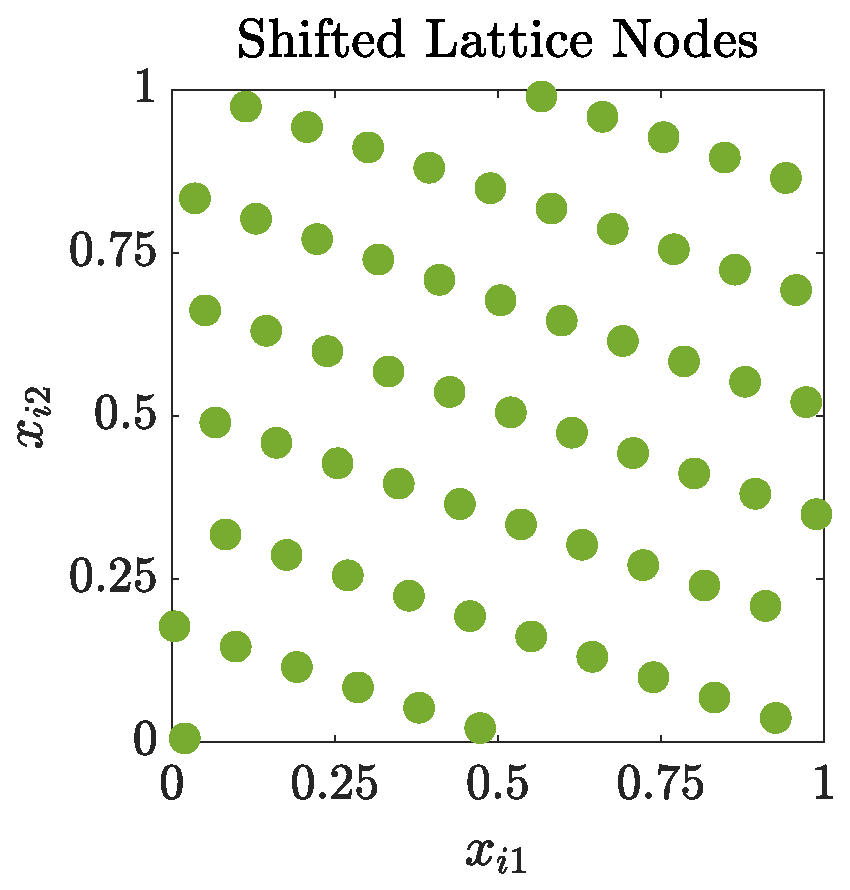
\includegraphics[width=3cm]{ProgramsImages/ShiftedLatticePoints.eps} \qquad
    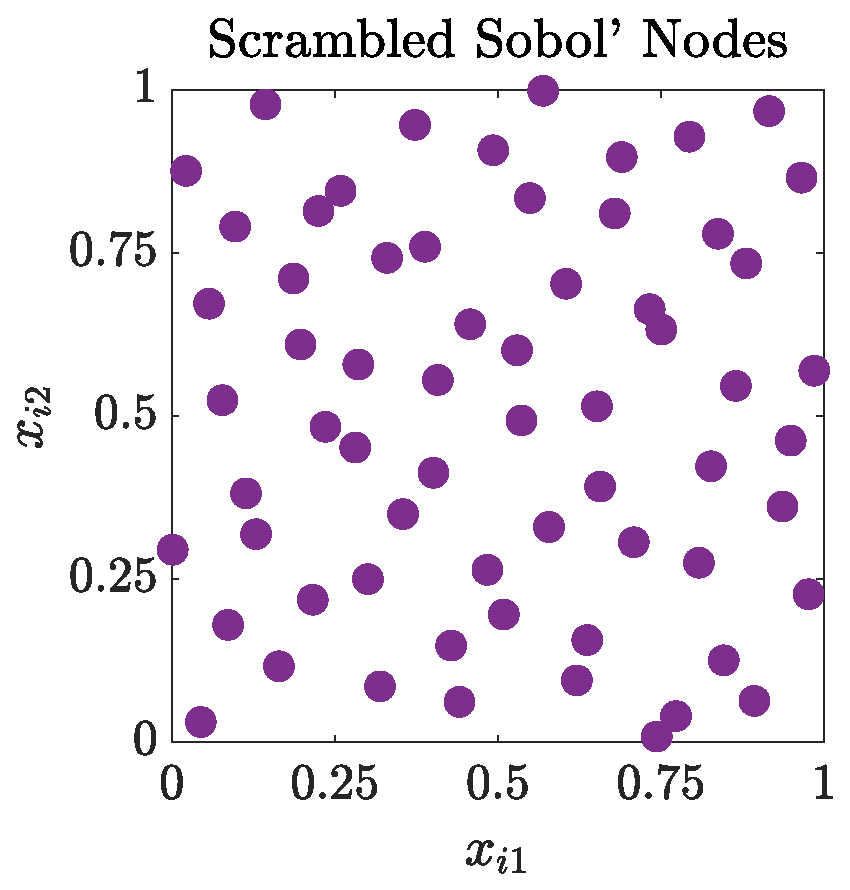
\includegraphics[width=3cm]{ProgramsImages/SSobolPoints.eps}}
\end{align*}

\end{frame}

\begin{frame}{Complex Exponential and Walsh Bases for Cubature}
\vspace{-3ex}
	\begin{tabular}{>{\centering}m{0.18\textwidth}>{\centering}m{0.18\textwidth}>{\centering}m{0.18\textwidth}>{\centering}m{0.18\textwidth}>{\centering}m{0.18\textwidth}}
		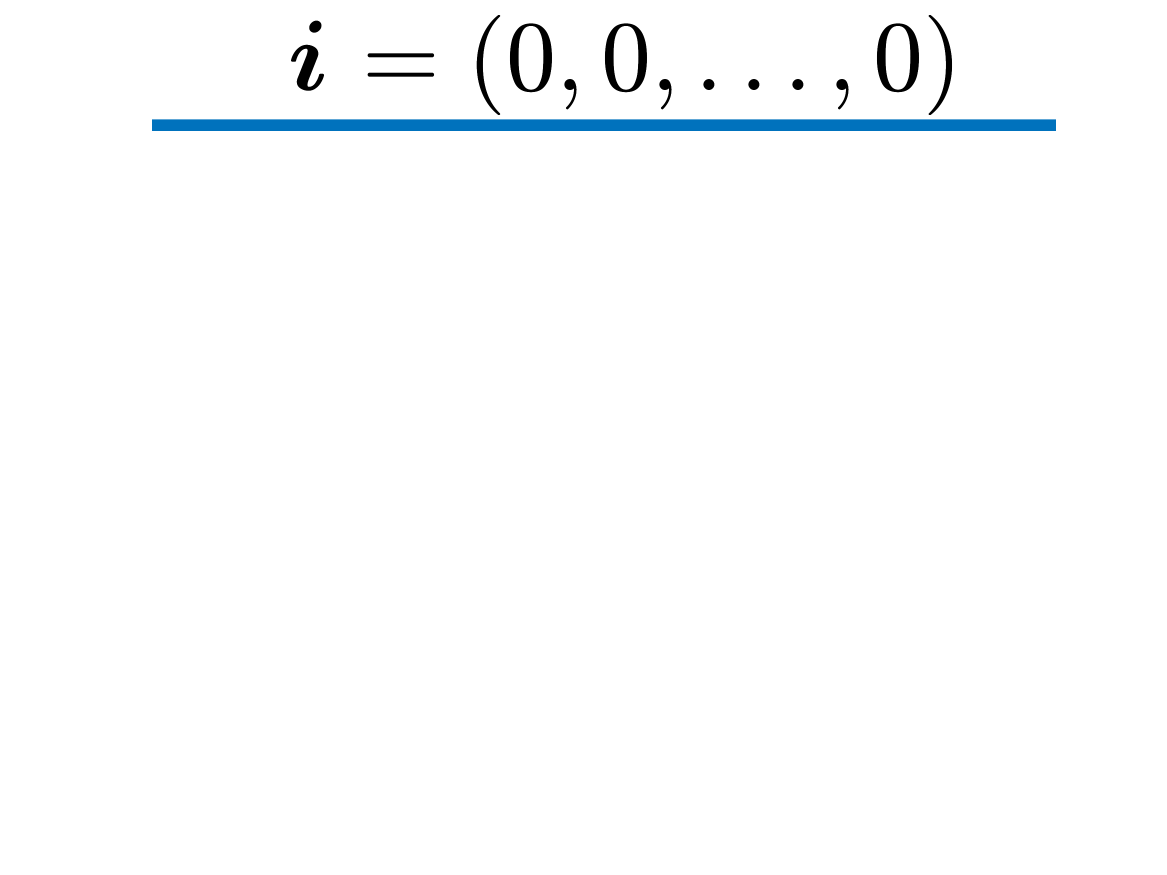
\includegraphics[width =0.18\textwidth]{ProgramsImages/CosineSine_Degree_0.png}  &
		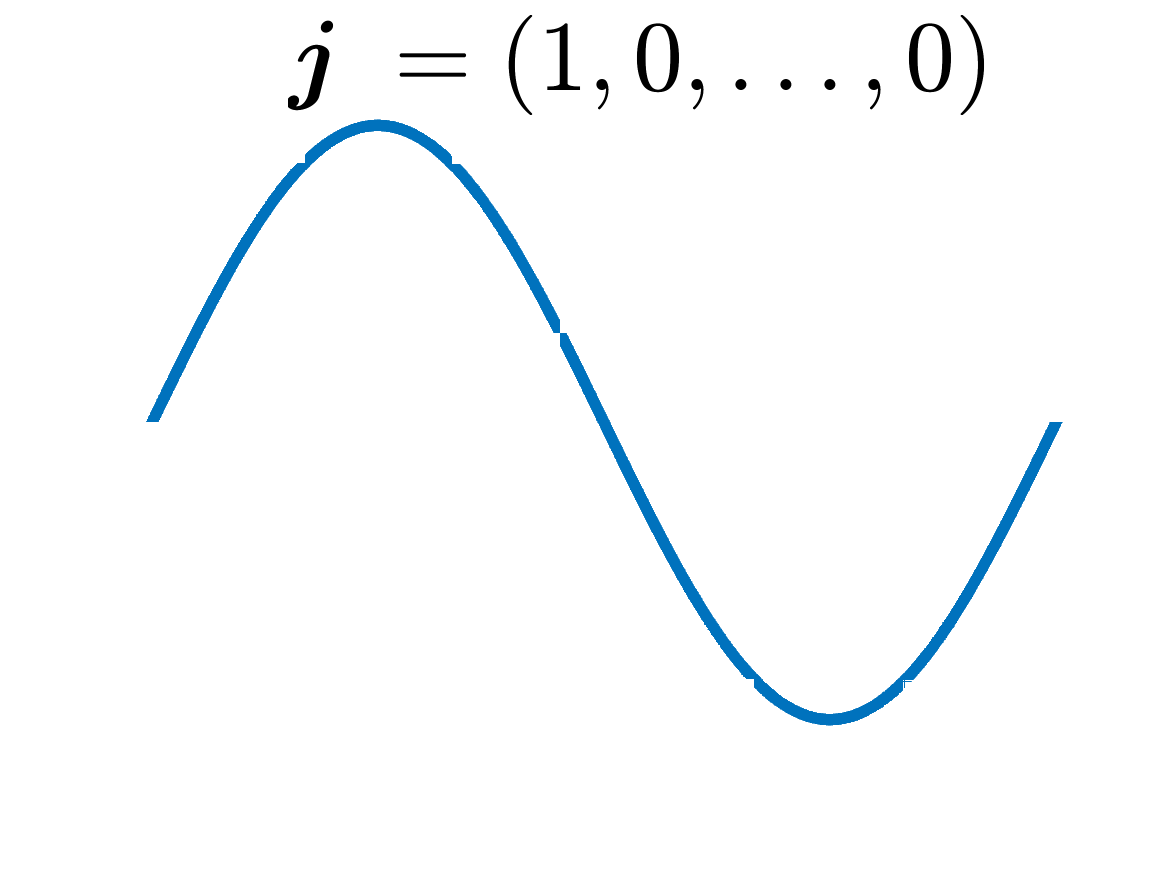
\includegraphics[width =0.18\textwidth]{ProgramsImages/CosineSine_Degree_1.png}  &
		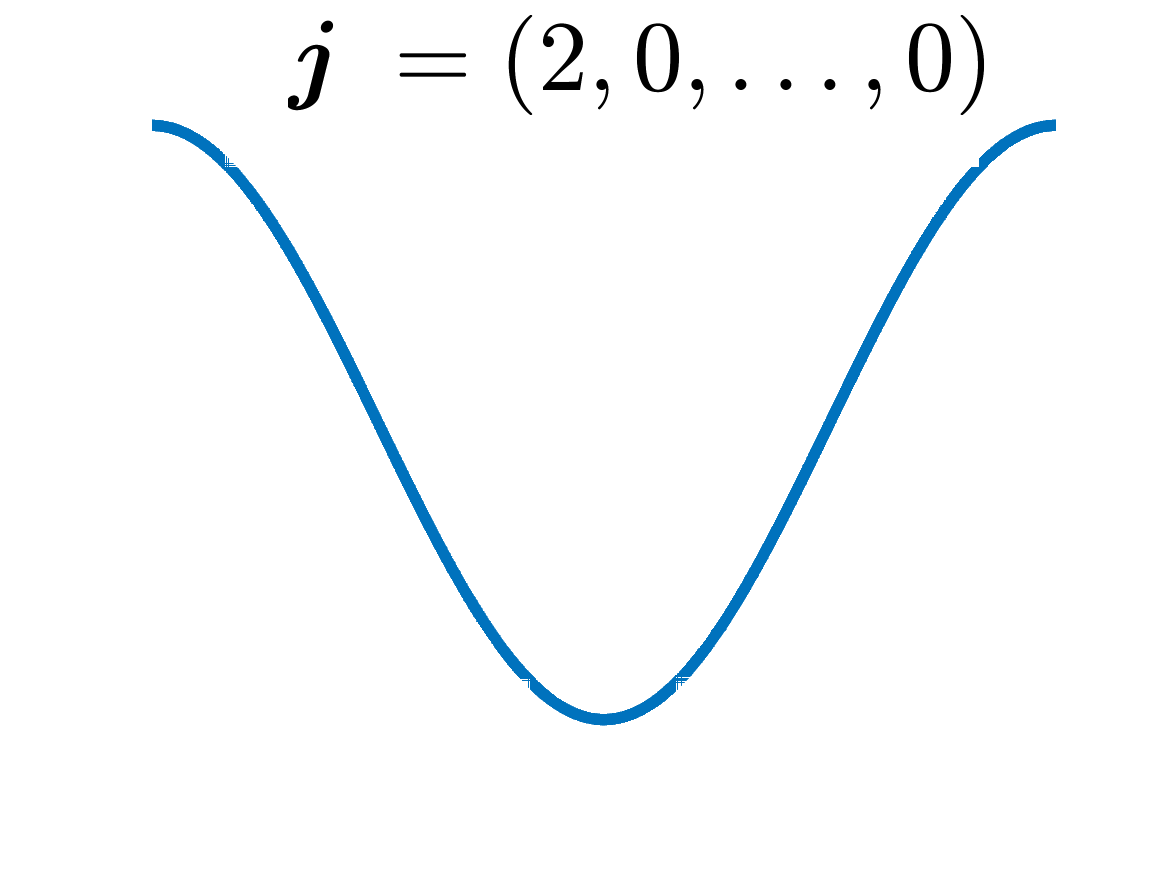
\includegraphics[width =0.18\textwidth]{ProgramsImages/CosineSine_Degree_2.png}  &
		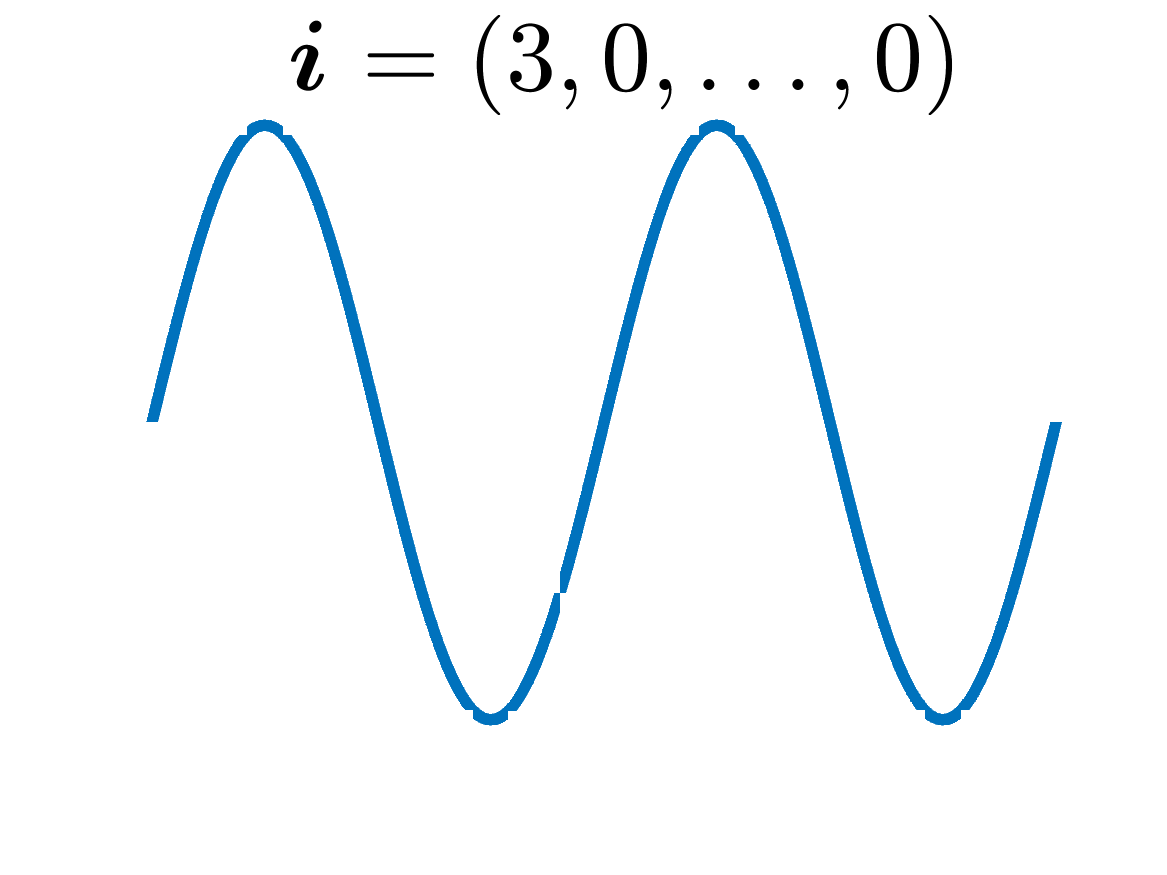
\includegraphics[width =0.18\textwidth]{ProgramsImages/CosineSine_Degree_3.png}  &
		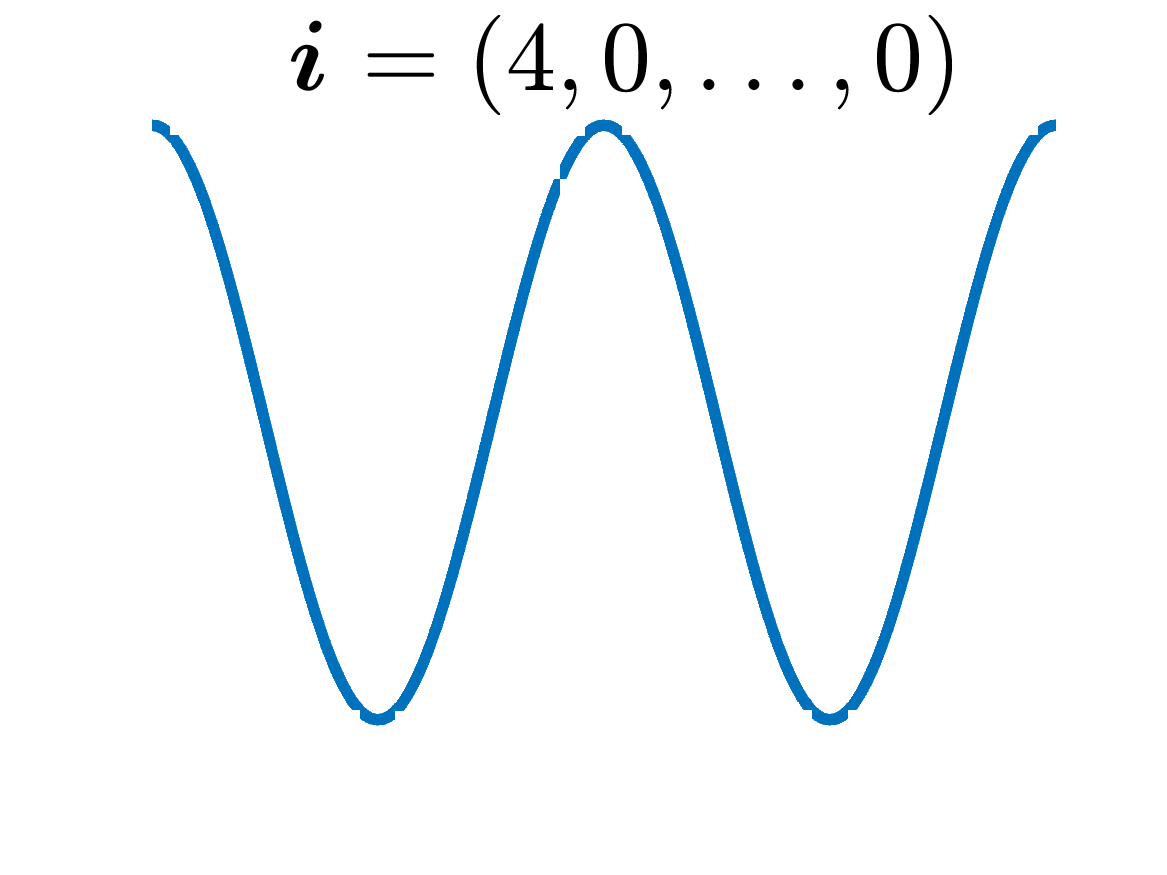
\includegraphics[width =0.18\textwidth]{ProgramsImages/CosineSine_Degree_4.png} 
	\tabularnewline[-7ex]
	Cosine \& Sine
	\tabularnewline
	\tabularnewline
		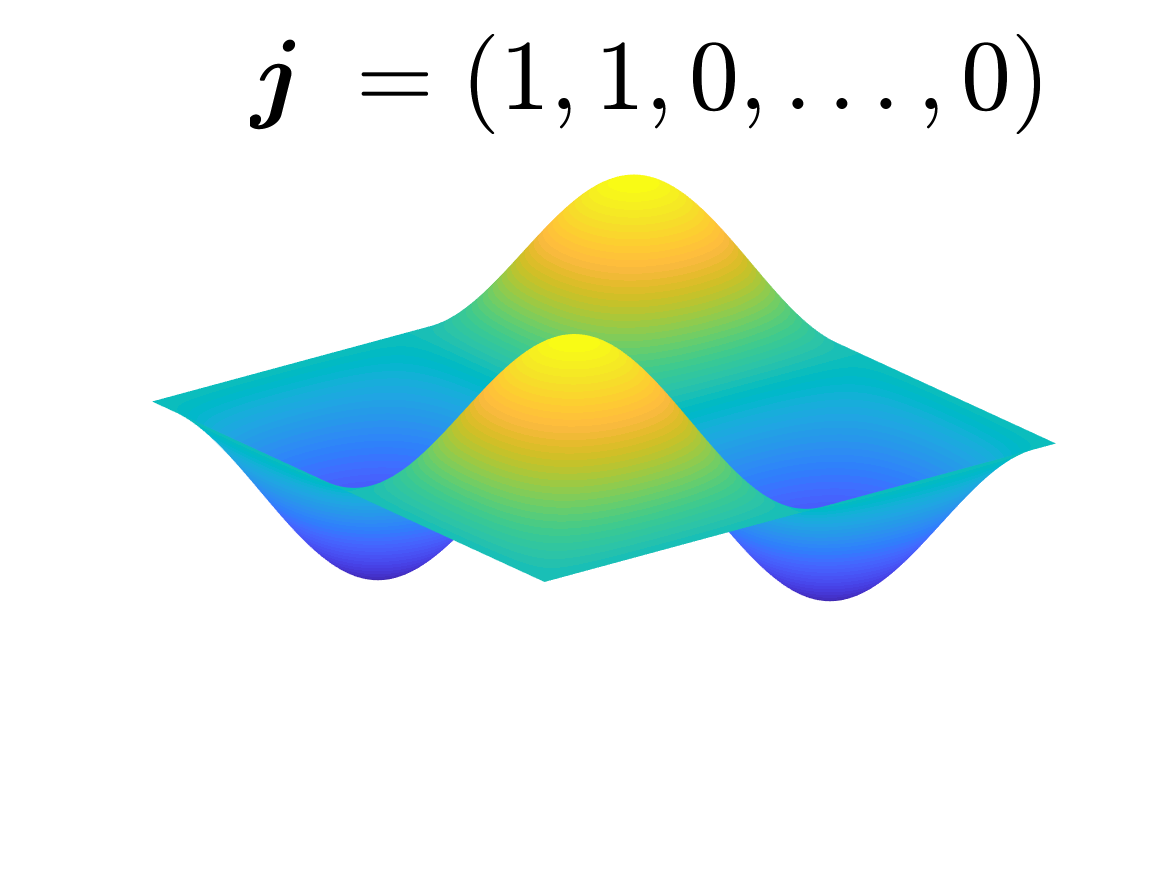
\includegraphics[width =0.18\textwidth]{ProgramsImages/CosineSine_Degree_1_1.png}  &
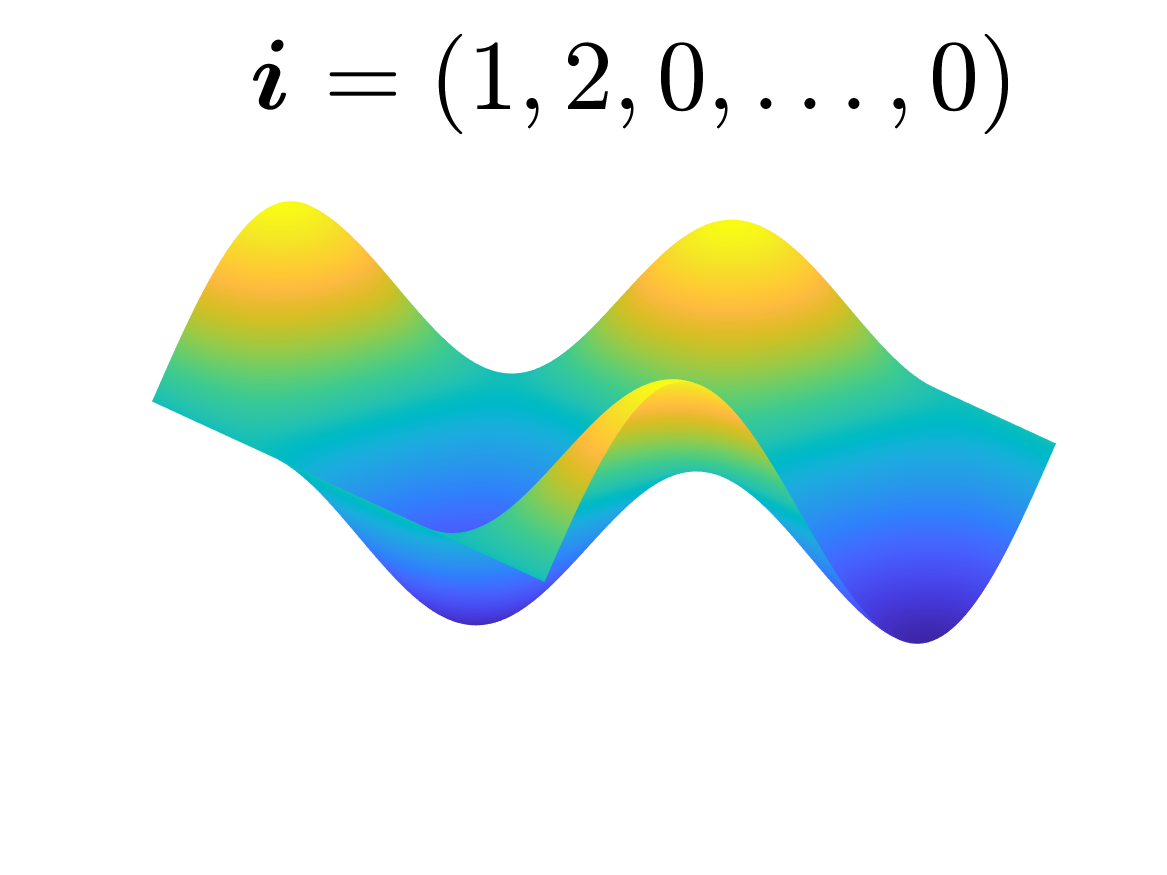
\includegraphics[width =0.18\textwidth]{ProgramsImages/CosineSine_Degree_1_2.png}  &
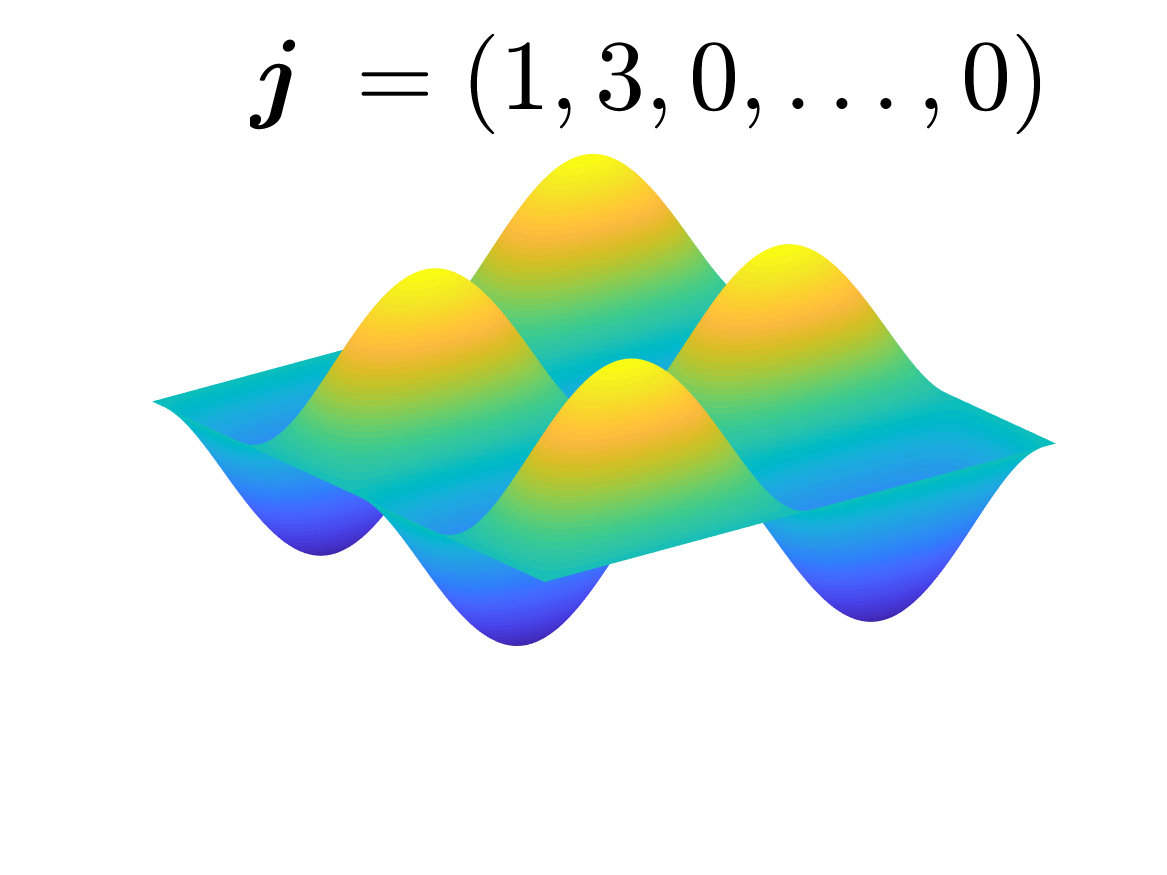
\includegraphics[width =0.18\textwidth]{ProgramsImages/CosineSine_Degree_1_3.png}  &
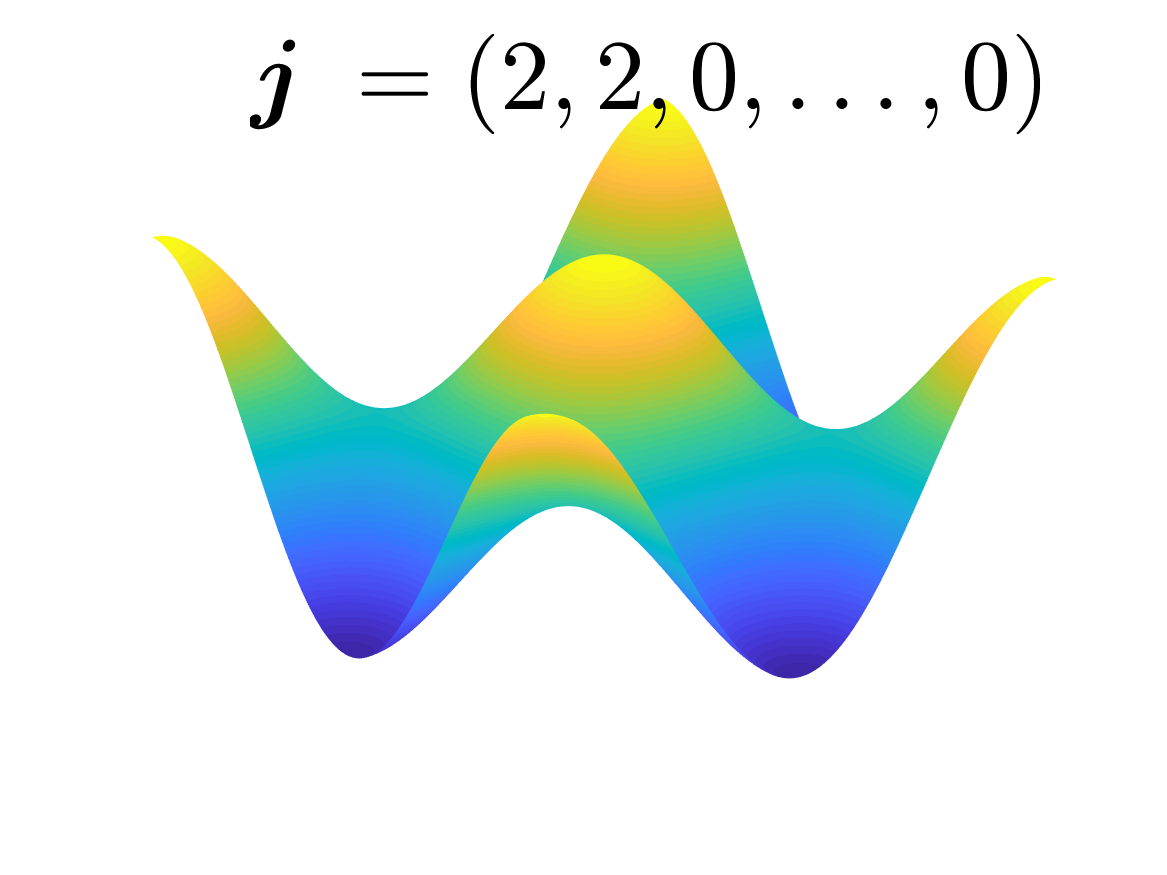
\includegraphics[width =0.18\textwidth]{ProgramsImages/CosineSine_Degree_2_2.png}  &
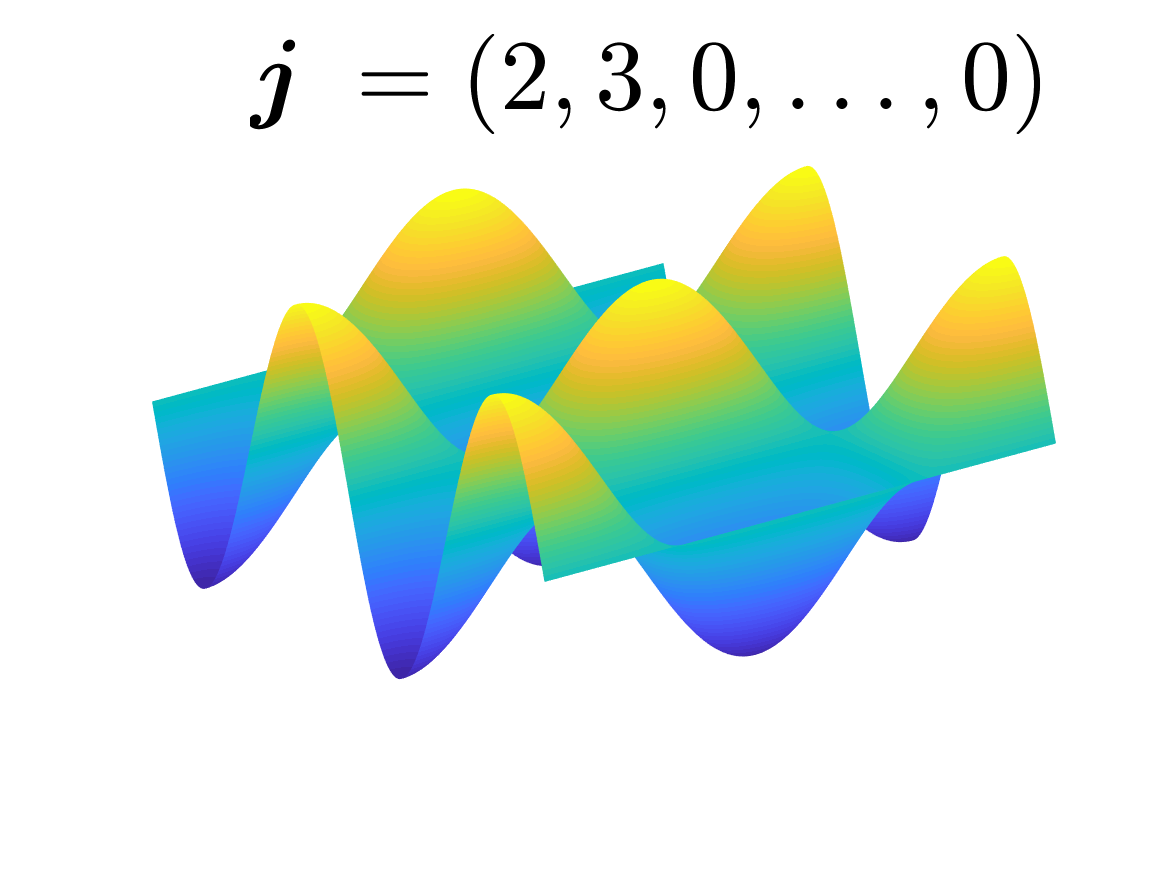
\includegraphics[width =0.18\textwidth]{ProgramsImages/CosineSine_Degree_2_3.png} 
\tabularnewline[0ex]
		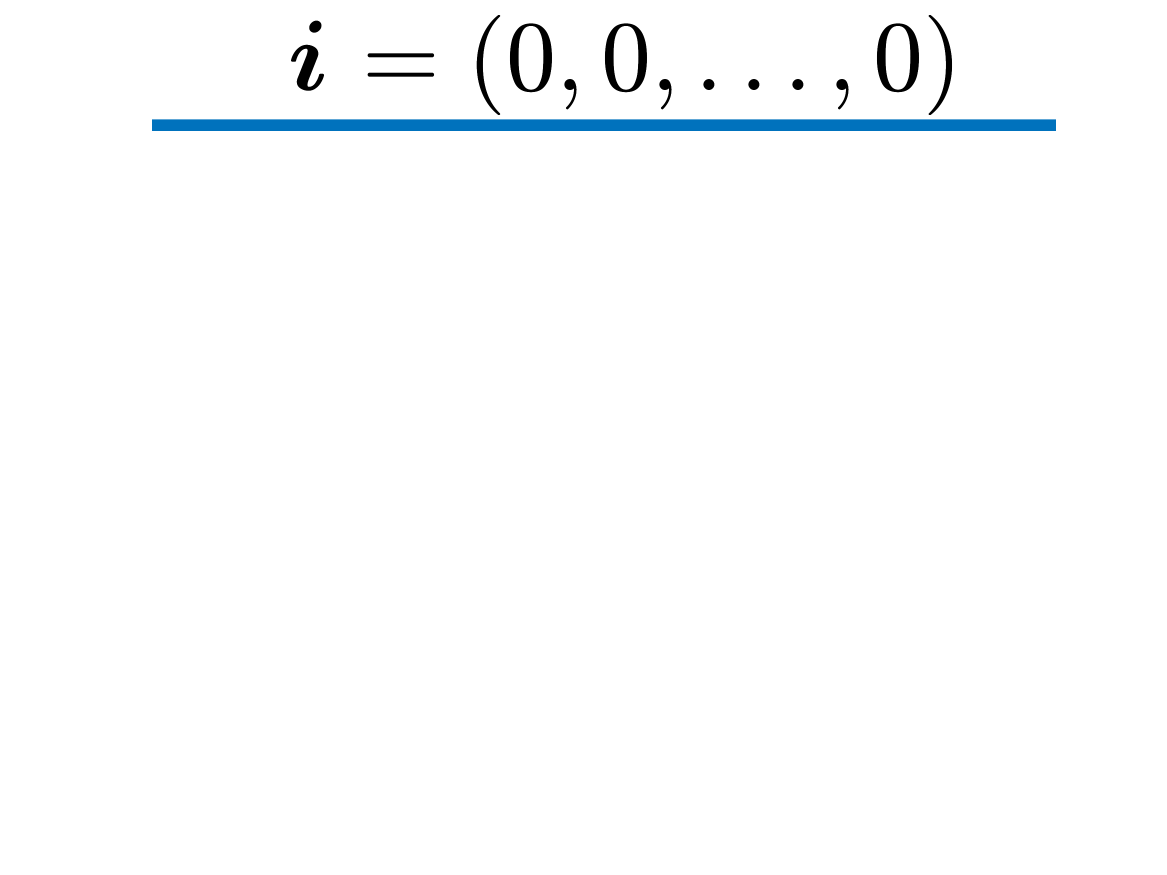
\includegraphics[width =0.18\textwidth]{ProgramsImages/Walsh_Degree_0.png}  &
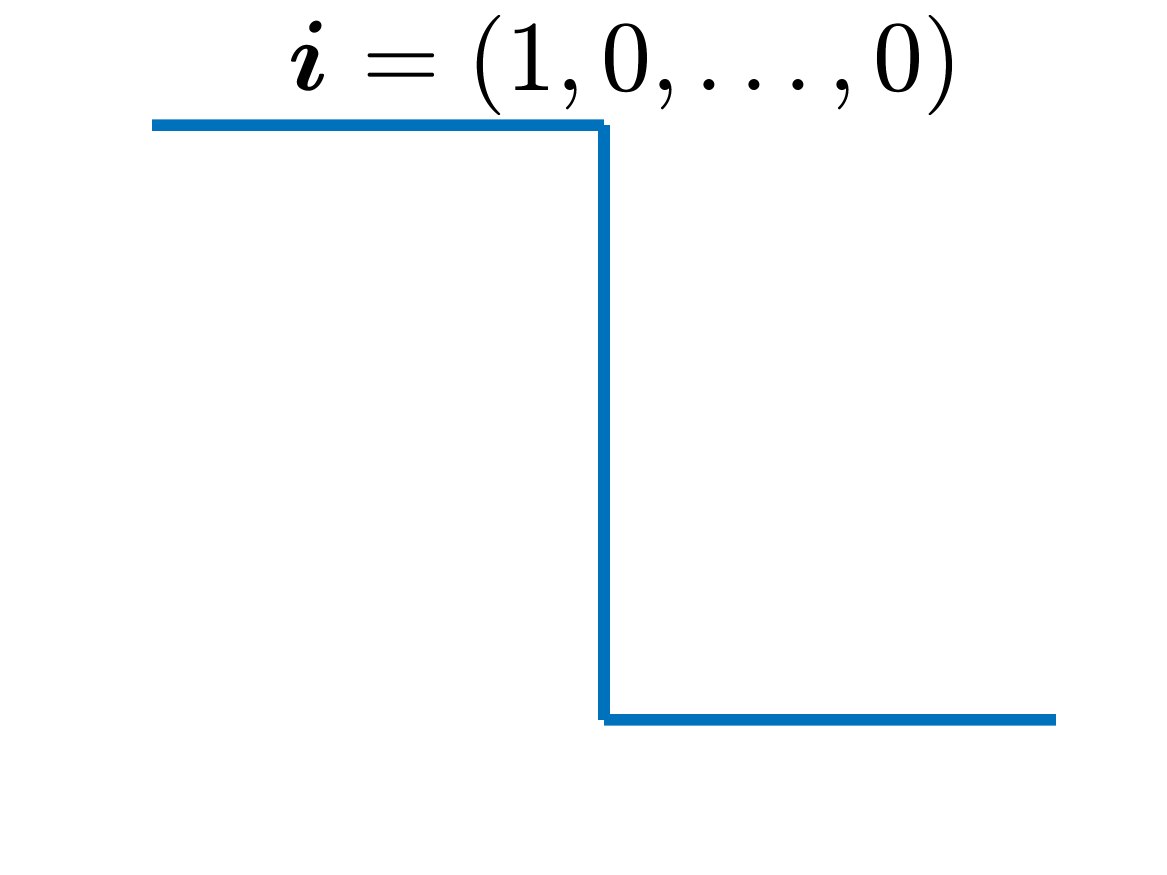
\includegraphics[width =0.18\textwidth]{ProgramsImages/Walsh_Degree_1.png}  &
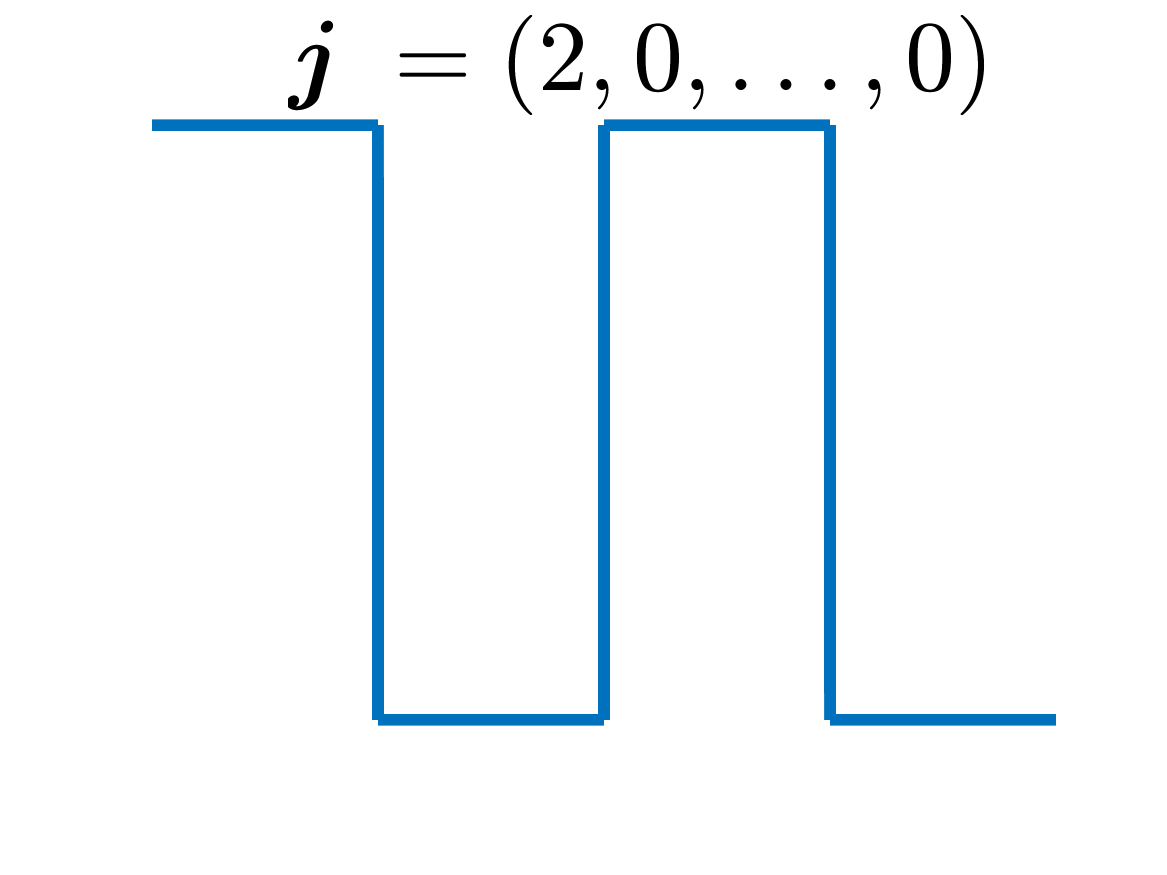
\includegraphics[width =0.18\textwidth]{ProgramsImages/Walsh_Degree_2.png}  &
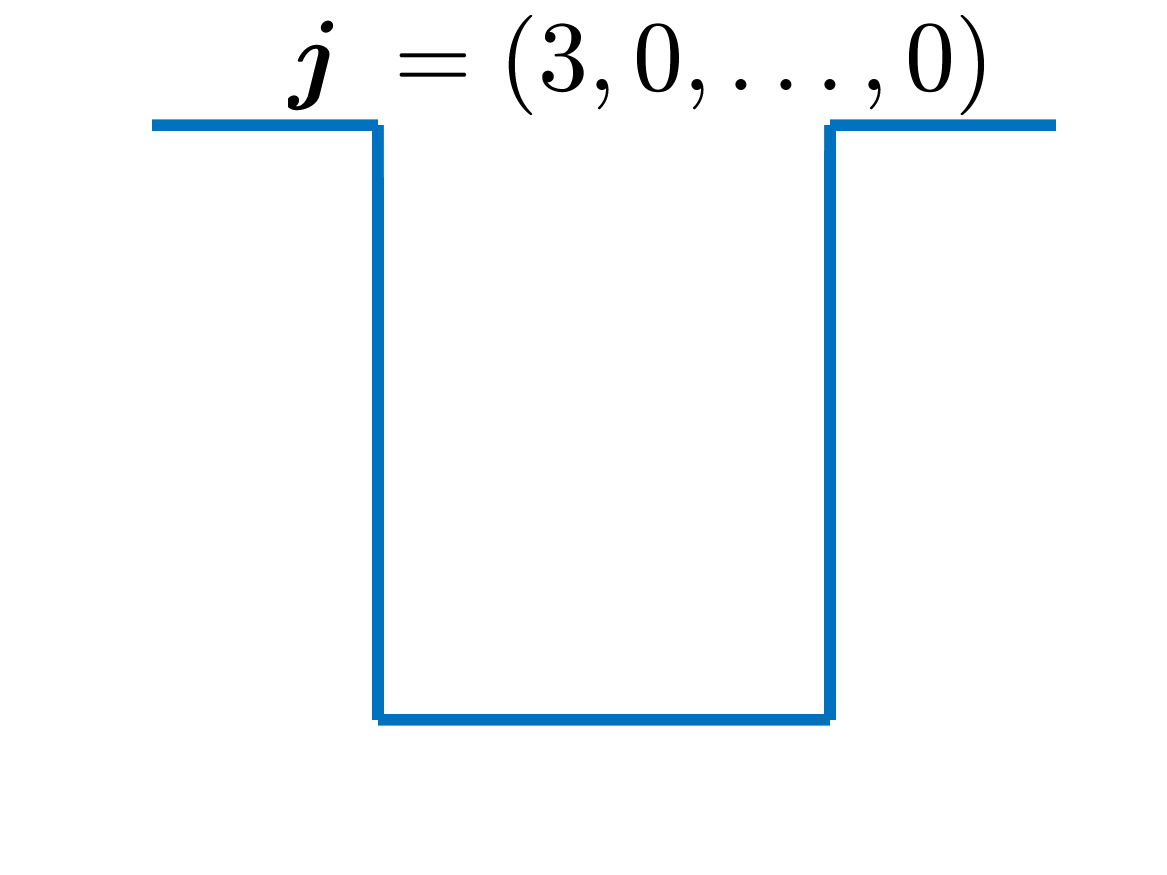
\includegraphics[width =0.18\textwidth]{ProgramsImages/Walsh_Degree_3.png}  &
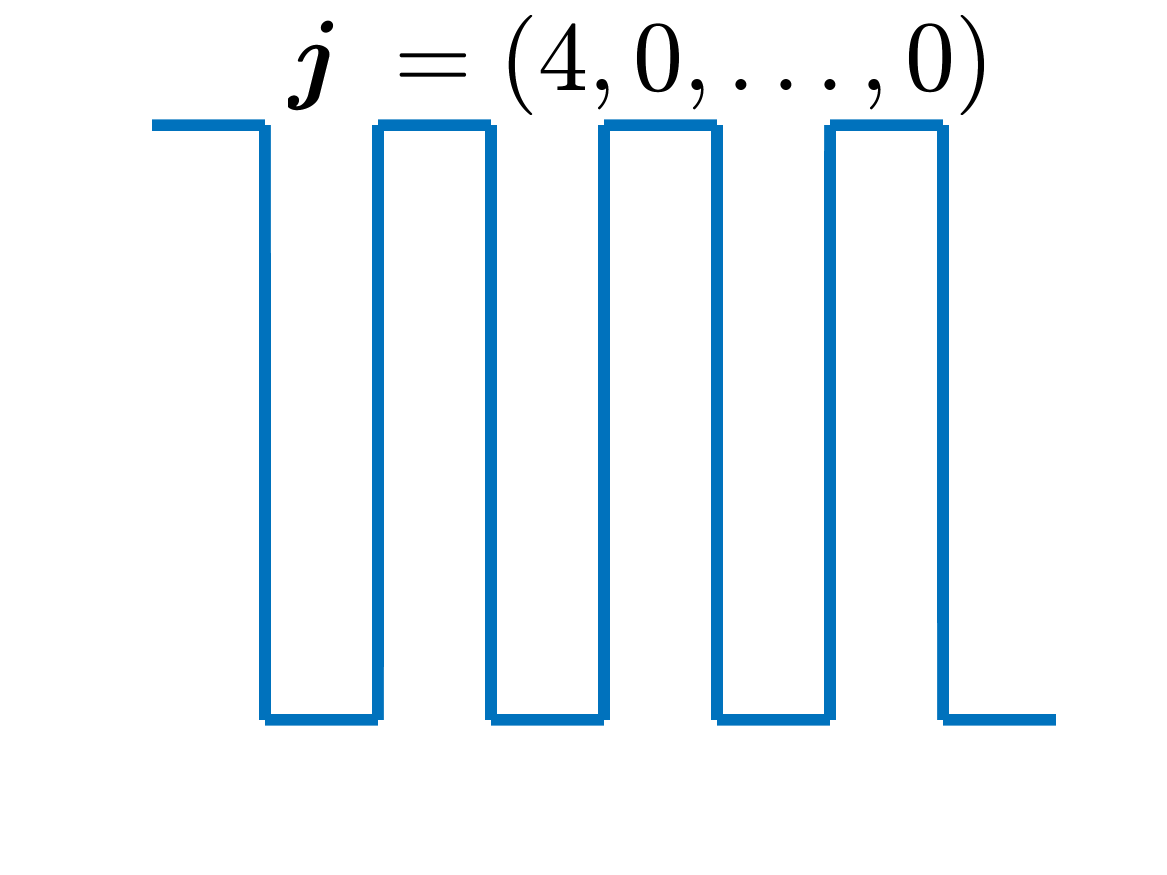
\includegraphics[width =0.18\textwidth]{ProgramsImages/Walsh_Degree_4.png} 
\tabularnewline[-7ex]
Walsh \tabularnewline
\tabularnewline
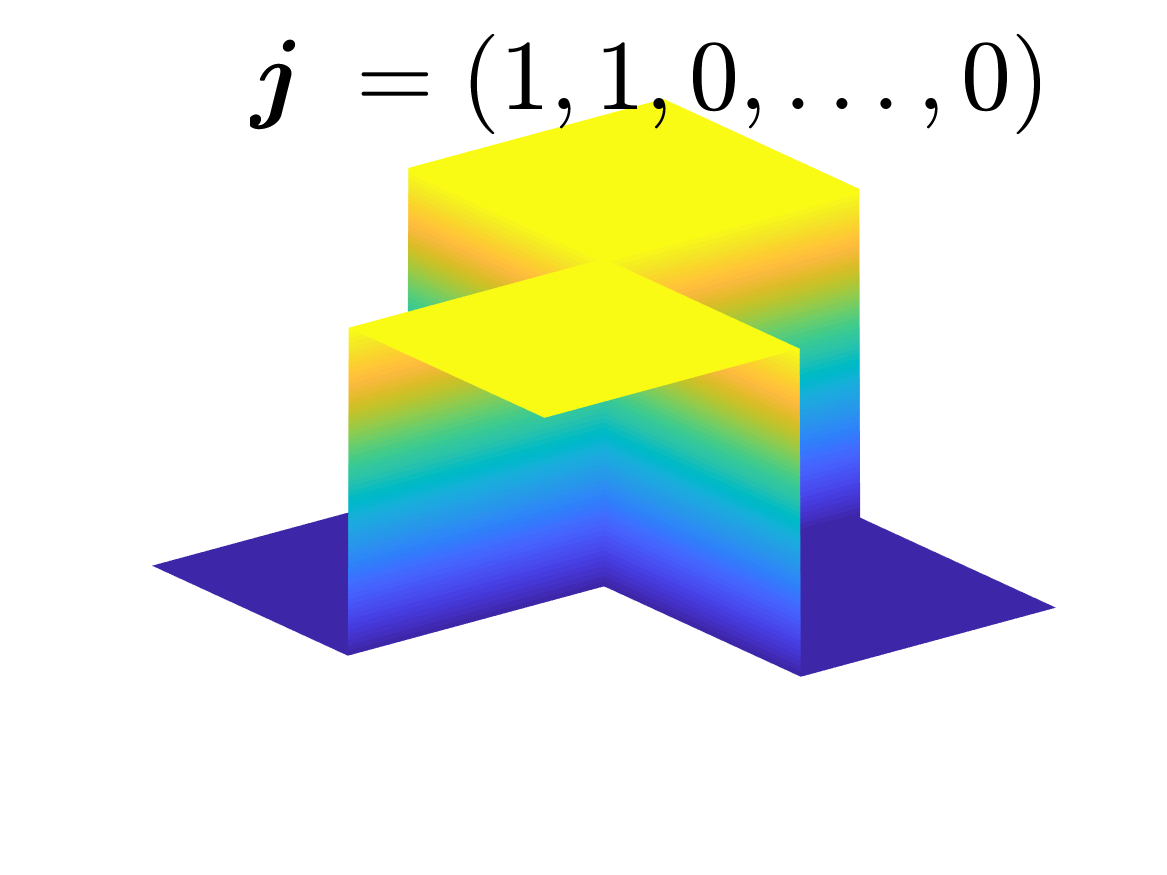
\includegraphics[width =0.18\textwidth]{ProgramsImages/Walsh_Degree_1_1.png}  &
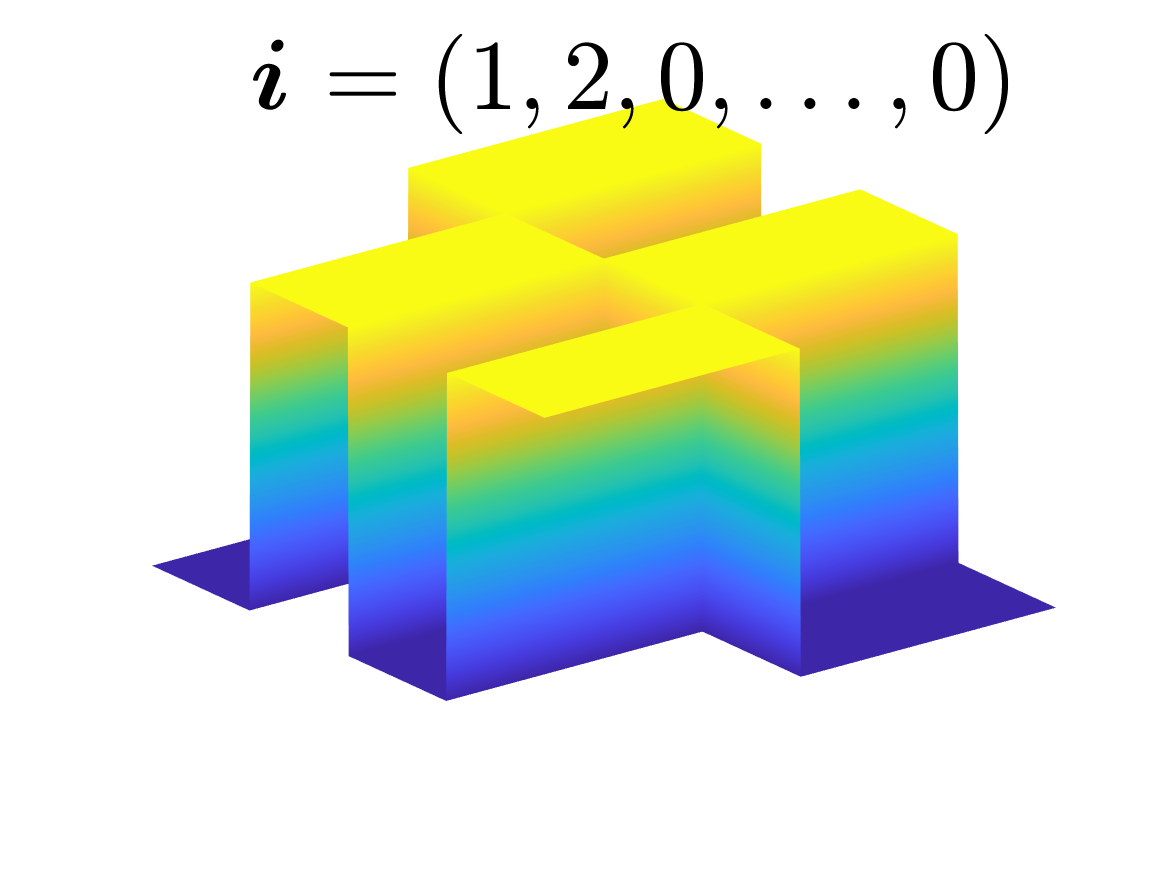
\includegraphics[width =0.18\textwidth]{ProgramsImages/Walsh_Degree_1_2.png}  &
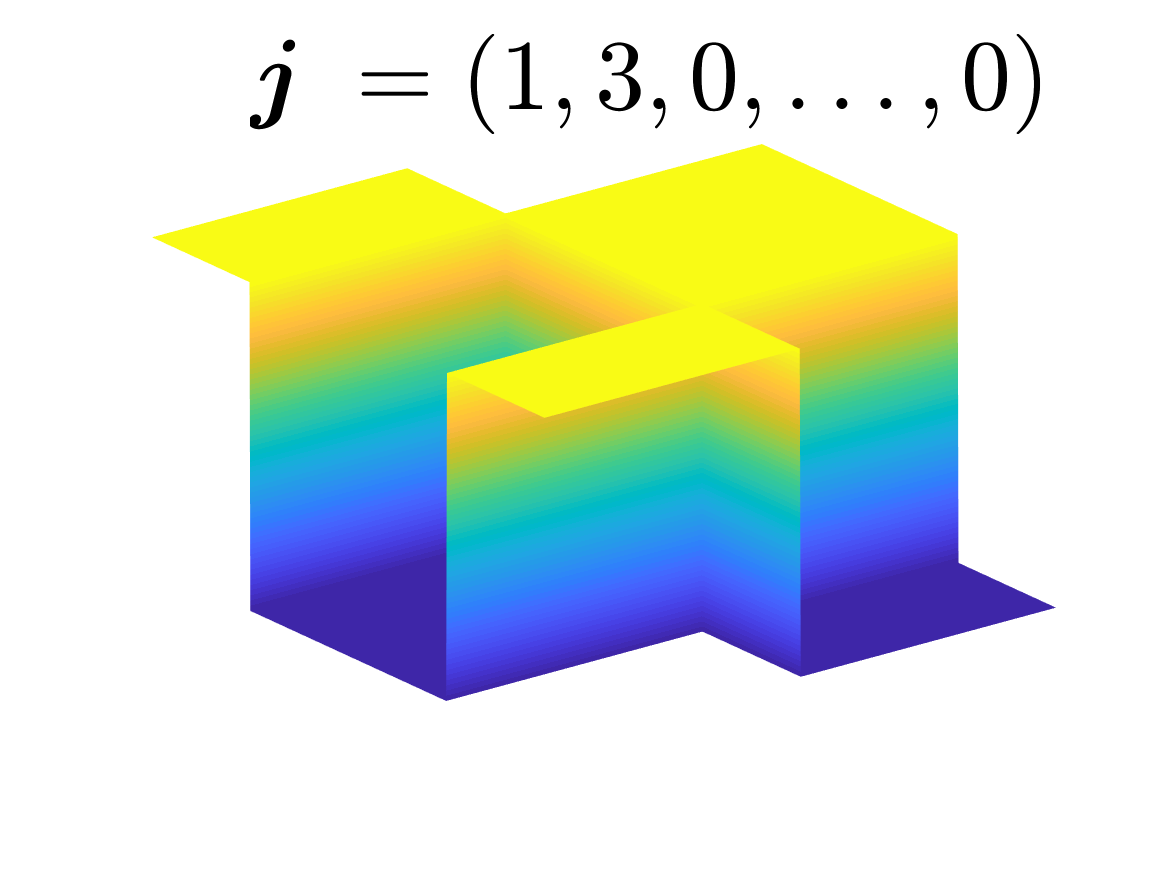
\includegraphics[width =0.18\textwidth]{ProgramsImages/Walsh_Degree_1_3.png}  &
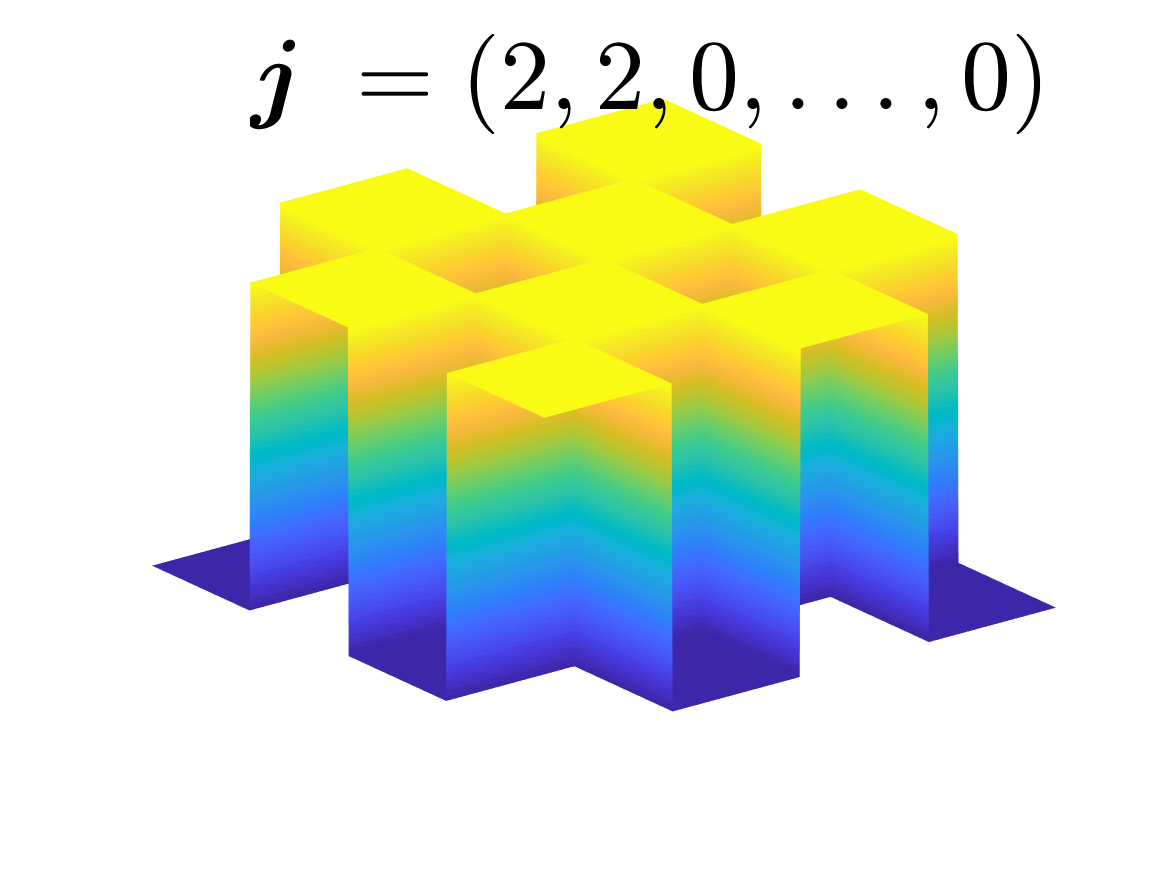
\includegraphics[width =0.18\textwidth]{ProgramsImages/Walsh_Degree_2_2.png}  &
\includegraphics[width =0.18\textwidth]{ProgramsImages/Walsh_Degree_2_3.png} 
	\end{tabular}
\end{frame}



\begin{frame}{Cones of Integrands Whose Fourier Series Coefficients Decay Steadily\footfullcite{HicJim16a,JimHic16a}}

\vspace{-8ex}

\begin{align*}
n_0 & = 0, \quad n_k = 2^{k-1}, \ k \in \naturals, \qquad \vj \text{ ordered}, \quad \text{true coef.} = \hf(\vj) \approx \hf_{\text{disc}}(\vj) = \text{discrete coef.}\\
	 \sigma_k(f) & = \sum_{i=n_{k-1}+1}^{n_k}  \bigabs{\hf(\vj_i)}, \quad  \hsigma_{k,\ell}(f)  = \sum_{i=n_{k-1}+1}^{n_k} \sum_{m=1}^{\infty} \bigabs{\hf(\vj_{i+mn_{\ell}})}, \quad \sigma_{\textup{disc},k}(f) = \sum_{i=n_{k-1}+1}^{n_k}  \bigabs{\hf_{\text{disc}}(\vj_i)} \\
	 \cc &: = \left\{f \in \cf :  
	 \sigma_\ell(f) \le a_1 b_1^{\ell - k}\sigma_k(f), \   \hsigma_{k,\ell}(f) \le a_2 b_2^{\ell - k} \sigma_\ell(f) \quad \forall k \le \ell \right\} \quad a_1, a_2 > 1 > b_1, b_2\\
      \MoveEqLeft{\Sapp(f,n_k) = \frac 1{n_k} \sum_{i=1}^{n_k} f(\vx_i)  \quad
    \abs{S(f) - \Sapp(f,n_k)} \le \sum_{\vzero \ne \vj \in \text{dual set}} \bigabs{\hf(\vj)} \le C(k) \sigma_{\textup{disc},k}(f)} \\
    \alert{A(f,\varepsilon)} & \alert{= S(f,n_k) \text{ for the smallest $k$ satisfying } C(k) \sigma_{\textup{disc},k}(f) \le \varepsilon}
\end{align*}

\vspace{-4ex}
\alert{Have} $\COST(f,A,\varepsilon)$; \quad \alert{No} $\COST(A,\cc,\varepsilon,\rho)$,  $\comp(\ca(\cc,\LambdaStd),\varepsilon,\rho)$, or  tractability results \alert{yet}

\end{frame}

\begin{frame}
\frametitle{Integrands in $\cc$ Aren't Fuzzy}

\setlength{\figwidth}{0.4\textwidth}

\vspace{-6ex}


\centerline{
	\includegraphics[width = \figwidth] 
	{ProgramsImages/FunctionWalshFourierCoeffDecay.eps} \qquad \qquad
	\includegraphics[width = \figwidth] 
	{ProgramsImages/FilteredFunctionWalshFourierCoeffDecay.eps} }


\end{frame}


\begin{frame}{ Option Pricing\footfullcite{ChoEtal17b}}
\vspace{-12ex}
\begin{tabular}{m{11cm}m{2.5cm}}
	\[
	\begin{aligned}
	 \text{fair price} = 
	\int_{\reals^d}\me^{-r T}\max\left(\frac{1}{d}\sum_{j=1}^d S_{j}-K, 0\right) 
	\frac{\me^{-\vz^T\vz/2}}{(2\pi)^{d/2}}\,\dif \vz \approx \$13.12
	\end{aligned}
	\]
	& 
	\financePict
\end{tabular}
\vspace{-4ex}
\begin{gather*}
S_{j} =  S_0\me^{(r-\sigma^2/2)jT/d+\sigma x_j} = \text{stock price at time } 
jT/d, \\
\vx  = \mA \vz, \quad \mA \mA^T = \mSigma = \Bigl ( \min(i,j) T/d \Bigr) _{i,j = 1}^d,
\quad T = 1/4, \ d=13 \text{ here}
\end{gather*}
\begin{equation*}
\begin{array}{cccccccc}
\text{Error}& && \text{Median}&& \text{Worst 10\%} & \text{Worst 10\%} \\
\text{Tolerance} & \multicolumn{2}{c}{\text{Method}}  & \text{Error} & \text{Accuracy} 
& n & \text{Time (s)} \\
\toprule
\input{ProgramsImages/AsianOutput.txt}
\end{array}
\end{equation*}
\vspace{-8ex}

\end{frame}

\begin{frame}{To Do List for Integration}

\begin{itemize}

\item My presentation here is a bit different than the original papers; we should check that the theory in those papers still go through (\alert{Fred})
    \item Find a norm on $\cf$ that allows us to prove results about computational complexity, optimality, and tractability.
    
    \item Hard to relate the \smallcone definition to Korobov spaces traditionally used for integration problems
    
\end{itemize}
    
\end{frame}


\section{General Linear Problems}

\begin{frame}{Solving General Linear Problems Using Series Coefficients, $\LambdaSer$\footfullcite{DinHic20a}}

\vspace{-7ex}

\begin{align*}
    \only<1>{\cf &:= \left \{ f = \sum_{\vk \in \cn} \hf(\vk) u_{\vk} : \norm[\cf]{f} := \norm[2]{\left(\frac{\bigabs{\hf(\vk)}}{\lambda_{\vk}} \right)_{\vk \in \cn}} \right \} \qquad \begin{minipage}{3cm}\raggedright\alert{$\vlambda$ affects convergence rate \& tractability}\end{minipage}\\
    \cg &: = \biggl \{ g = \sum_{\vk \in \cn} \hg(\vk) v_{\vk} : \norm[\cg]{g} := \bignorm[2]{\hg}\biggr \}, \qquad v_{\vk} = S(u_{\vk}) \\[-2ex]}
      & \alert{\lambda_{\vk_1} \ge \lambda_{\vk_2} \ge \cdots}, \qquad
      n_0 < n_1 < n_2 < \cdots,  \qquad
 	\sigma_k(f) = \sqrt{\sum_{i=n_{k-1}+1}^{n_k}  \bigabs{\hf(\vk_i)}^2}, \quad k \in \naturals \\
     \cc &: = \left\{f \in \cf :  
 	 \sigma_\ell(f) \le a b^{\ell - k}\sigma_k(f) \quad \forall k \le \ell \right\} \quad a > 1 > b \quad \text{\alert{series coef.\ decay steadily}}\\
 	 \Sapp(f,n_k) &= \sum_{i=1}^{n_k} \hf(\vk_i) v_{\vk_i} \text{ is optimal for fixed }n_k, \qquad \norm[\cg]{S(f) - \Sapp(f,n_k)} \le \frac{ab \sigma_k(f)}{\sqrt{1 - b^2}} \\[-1ex]
 	 \alert{A(f,\varepsilon)} & \alert{= \Sapp(f,n_k)} \text{ for the smallest $k$ satisfying } \alert{\sigma_k(f) \le \frac{\varepsilon \sqrt{1 - b^2}}{ab}}
 	 \only<2>{\\ 
 	 \MoveEqLeft{\alert{\COST(A,\cc,\varepsilon,\rho) = n_{\ell^\dagger}}, \quad 
 	 \ell^\dagger \le \min \left \{\ell \in \naturals : \frac{\rho^2}{\varepsilon^2} \le \frac{(1 - b^2)}{a^2b^2} \left[ \sum_{k=1}^{\ell-1} \frac{b^{2(k-\ell)}}{a^2\lambda_{n_{k-1}+1}^2} + \frac{1}{\lambda_{n_{\ell-1}+1}^2}\right]   \right\}} \\
 	 \MoveEqLeft{\COST(A,\cc,\varepsilon,\rho) \text{ \alert{essentially no worse than} } \comp(\ca(\cc,\LambdaAll),\varepsilon,\rho)}\\
 	 \MoveEqLeft{\text{\alert{No} tractability results}}}
\end{align*}

\end{frame}

\begin{frame}{To Do List for General Linear Problems}

\begin{itemize}

\item Shall we try general Banach spaces instead of only Hilbet spaces (\alert{Yuhan})
    \item Tractability should not be a big problem (\alert{Peter, Yuhan})
    
    \item Need to define $\lambda_\vj$ in terms for tensor product spaces (\alert{Peter, Yuhan})
    
\end{itemize}
    
\end{frame}



\section{Function Approximation}

\begin{frame}{\emph{Function Approximation} when Function Values Are Expensive\footfullcite{WuHam00,KuoEtal12a}}

\vspace{-7ex}

    \begin{align*}
    \only<1>{\cf &:= \left \{ f = \sum_{\vj \in \natzero^d} \hf(\vj) u_{\vj} : \norm[\cf]{f} :=  \norm[\infty]{\left(\frac{\bigabs{\hf(\vj)}}{\lambda_{\vj}} \right)_{\vj \in \cn}} \right \} \qquad \begin{minipage}{3cm}\raggedright\alert{$\vlambda$ affects convergence rate \& tractability}\end{minipage}\\
    \cg &: = \Biggl \{ g = \sum_{\vj \in \natzero^d} \hg(\vj) v_{\vj} : \norm[\cg]{g} := \bignorm[1]{\hg}\Biggr \}, \qquad v_{\vj} = S(u_{\vj}) = u_{\vj} \\[-2ex]}
    \lambda_{\vj} & = \Gamma_{\norm[0]{\vj}} \prod_{\substack{\ell = 1 \\ j_{\ell} > 0}}^d \gamma_\ell s_{j_\ell} \quad
    \begin{cases}
\gamma_\ell = \text{coordinate importance} \\[-0.5ex]
\Gamma_r = \text{order size} \\[-0.5ex]
s_j =  \text{smoothness degree}
\end{cases} \quad\begin{minipage}{5.5cm}\raggedright\alert{POSD weights reflect effect sparsity, effect hierarchy, effect heredity, and effect smoothness}\end{minipage}
 \\[-2ex]
      & \alert{\lambda_{\vj_1} \ge \lambda_{\vj_2} \ge \cdots}, \qquad
      \Sapp(f,n) = \sum_{i=1}^{n} \hf(\vj_i) u_{\vj_i} ,  \qquad
 	\norm[\cg]{S(f) - \Sapp(f,n_k)} \le \norm[\cf]{f} \sum_{i = n+1} \lambda_{\vj_i} \\
     \cc &: = \left\{f \in \cf :  \text{ those functions for which } \norm[\cf]{f} \text{ can be \alert{inferred} from a pilot sample} \right \}
\end{align*}

\end{frame}

\begin{frame}{Legendre and Chebyshev Bases for Function Approximation}
\vspace{-3ex}
	\begin{tabular}{>{\centering}m{0.18\textwidth}>{\centering}m{0.18\textwidth}>{\centering}m{0.18\textwidth}>{\centering}m{0.18\textwidth}>{\centering}m{0.18\textwidth}}
		\includegraphics[width =0.18\textwidth]{ProgramsImages/Legendre_Degree_0.png}  &
		\includegraphics[width =0.18\textwidth]{ProgramsImages/Legendre_Degree_1.png}  &
		\includegraphics[width =0.18\textwidth]{ProgramsImages/Legendre_Degree_2.png}  &
		\includegraphics[width =0.18\textwidth]{ProgramsImages/Legendre_Degree_3.png}  &
		\includegraphics[width =0.18\textwidth]{ProgramsImages/Legendre_Degree_4.png} 
	\tabularnewline[-7ex]
	Legendre
	\tabularnewline
	\tabularnewline
		\includegraphics[width =0.18\textwidth]{ProgramsImages/Legendre_Degree_1_1.png}  &
\includegraphics[width =0.18\textwidth]{ProgramsImages/Legendre_Degree_1_2.png}  &
\includegraphics[width =0.18\textwidth]{ProgramsImages/Legendre_Degree_1_3.png}  &
\includegraphics[width =0.18\textwidth]{ProgramsImages/Legendre_Degree_2_2.png}  &
\includegraphics[width =0.18\textwidth]{ProgramsImages/Legendre_Degree_2_3.png} 
\tabularnewline[0ex]
		\includegraphics[width =0.18\textwidth]{ProgramsImages/Chebyshev_Degree_0.png}  &
\includegraphics[width =0.18\textwidth]{ProgramsImages/Chebyshev_Degree_1.png}  &
\includegraphics[width =0.18\textwidth]{ProgramsImages/Chebyshev_Degree_2.png}  &
\includegraphics[width =0.18\textwidth]{ProgramsImages/Chebyshev_Degree_3.png}  &
\includegraphics[width =0.18\textwidth]{ProgramsImages/Chebyshev_Degree_4.png} 
\tabularnewline[-7ex]
Chebyshev \tabularnewline
\tabularnewline
\includegraphics[width =0.18\textwidth]{ProgramsImages/Chebyshev_Degree_1_1.png}  &
\includegraphics[width =0.18\textwidth]{ProgramsImages/Chebyshev_Degree_1_2.png}  &
\includegraphics[width =0.18\textwidth]{ProgramsImages/Chebyshev_Degree_1_3.png}  &
\includegraphics[width =0.18\textwidth]{ProgramsImages/Chebyshev_Degree_2_2.png}  &
\includegraphics[width =0.18\textwidth]{ProgramsImages/Chebyshev_Degree_2_3.png} 
	\end{tabular}
\end{frame}

\begin{frame}{Cheng and Sandu Function\footfullcite{VirLib17a}}
    \vspace{-9ex}
    \begin{gather*}
        \text{Chebyshev polynomials}, \qquad \text{Order weights }\Gamma_k = 1, \qquad \text{Coordinate weights } \gamma_\ell \text{ \alert{inferred}}, \\
        \text{Smoothness weights } s_j \text{ \alert{inferred}}, \qquad \LambdaStd
    \end{gather*}
    
    \vspace{-3ex}
    
    \includegraphics[height = 4.3cm]{ProgramsImages/sim_eval_results_chsan10_d6_sflg0ErrN.eps}
    \qquad \includegraphics[height = 4.3cm]{ProgramsImages/sim_eval_results_chsan10_d6_sflg0fErr.eps}
\end{frame}

\begin{frame}{To Do List for Function Approximation}

\begin{itemize}
    \item Determine the relationship between PODS weights and SPOD weights (\alert{Peter, Fred})
    
    \item Determine conditions on tractability; tensor product structure already built in (\alert{Peter})
    
    \item Need to try examples from Bingham's library and search for other examples (\alert{Simon})
    
    \item Need to bridge gap in theory between using $\LambdaSer$ and $\LambdaStd$ (\alert{Simon, Fred})
    
\end{itemize}
    
\end{frame}





\section{Summary}
\begin{frame}{Take Home Messages}

\vspace{-4ex}

\begin{itemize}
    \item Assuming that the input functions lie in convex \alert{cones} \smallcone allow us to construct \alert{adaptive} algorithms
    
    \item Cone definitions reflect \alert{prior beliefs} and/or \alert{practical considerations}
    
    \item Demonstration of concept
    \begin{itemize}
        \item Integration using $\LambdaStd$
        \begin{itemize}
            \item Constructed $A \in \ca(\cc,\LambdaStd)$
            \item No cost, complexity, or tractability yet
        \end{itemize}
        \item General linear problems
        \begin{itemize}
            \item Constructed $A \in \ca(\cc,\LambdaSer)$, upper bound on $\COST(A,\cc,\varepsilon,\rho)$, lower bound on $\comp(\ca(\cc,\LambdaAll),\varepsilon,\rho)$, optimality
            \item No tractability yet
        \end{itemize}
        \item Function approximation (recovery)
        \begin{itemize}
            \item Constructed $A \in \ca(\cc,\LambdaSer)$, algorithm learns weights, works in practice for $\LambdaStd$
            \item Remaining theory in progress
        \end{itemize}
    \end{itemize}
    
    \item Much to be done 
 
\end{itemize}
    
\end{frame}

\finalthanksnote{These slides are  available at \\  \href{https://speakerdeck.com/fjhickernell/ricam-2018-nov}{\nolinkurl{speakerdeck.com/fjhickernell/ricam-2018-nov}}}


\thankyouframe

\printbibliography

\section{Bonus}
\begin{frame}[label = VectorSpaceThmProof]{Proof of Theorem for Solvability on a Vector Space}

\vspace{-3ex}

Let the cone $\cc$ be a \alert{vector space} and let

\vspace{-3ex}
\begin{itemize}
    \item $A$ be a successful algorithm
    
    \item $\varepsilon > 0$ be any positive tolerance
    
    \item  $\{L_1, \ldots, L_{M}\} \subset \Lambda$ be the linear functionals used by $A(0,\varepsilon)$, and
    
    \item  $\{L_1, \ldots, L_m\}$ be a basis for $\spann(\{L_1, \ldots, L_{M}\})$
    
    \item $n  = \min(m,\dim(\cc))$
    
        \item $\{f_1, \ldots, f_n\} \subset \cc$ satisfy $L_i(f_j) = \delta_{i,j}$, $i =1, \ldots, n$, $j=1, \ldots, m$
\end{itemize}

\vspace{-2ex}

For any $f \in \cc$, let $\tf = f- \sum_{i=1}^n L_i(f) f_i$, and note that $L_j(\tf) = 0$ for $j =1, \ldots, M$.  Thus, $A(\tf,\varepsilon) = A(0,\varepsilon)$, and so by the \hyperlink{ZeroCorollary}{\beamergotobutton{Corollary}},
\[
0 = S(\tf) = S(f) - \sum_{i=1}^n L_i(f) S(f_i), \qquad \text{which implies } S(f) = \sum_{i=1}^n L_i(f) S(f_i)
\]

\vspace{-3ex}
    \hyperlink{VectorSpaceThm}{\beamerreturnbutton{Back}}
\end{frame}




\end{document}




